%!TEX root = ../thesis.tex
\chapter{Introduction}\label{cha:introduction}


\section{Towards the characterization of exoplanets}

The field of exoplanetary science is rapidly accelerating with large scientific and instrumental investments undertaken, with the ultimate goal of detecting and characterizing an Earth-like planet, with the potential for life (as we know it).
Since the very first exoplanet detection\footnote{around a Sun-like star}~\citep{mayor_jupitermass_1995} the number of confirmed\footnote{Validated by more than one detection method} exoplanets has grown to over 3790 with almost another 3000 candidates awaiting confirmation\footnote{\href{https://exoplanets.nasa.gov/}{exoplanets.nasa.govt} as of October 2018}.
However, simply detecting the presence of exoplanets is not nearly enough to satisfy our quest for knowledge.
There is an exorbitant amount to be gained through the full characterization of these known exoplanets: density, composition, internal structure, atmosphere properties, and surface temperature.

When an Earth-twin planet is suspected (there have been several false claims already \textbf{~\citep[e.g.][]{mullally_kepler_2018,}\textbf{ more}\todo{other dead earth-like planets} other earth like planets shown to not be earth like or redacted papers}) a full characterization is required to confirm it's habitability \textbf{(ref)}.
For instance, knowing only the mass and radius can provide an average density but not the composition or the internal structure~\textbf{ref}\citet{a paper about composition degeneracy}.
The presence of an exoplanet's atmosphere will also influence the average density but can provide detectable clues on the planet's composition.
Several techniques being explored to detect and characterize exoplanet atmospheres~\citep[e.g.][]{snellen_orbital_2010, martins_reflected_2016, piskorz_evidence_2016, } \textbf{a transmission spectroscopy paper} with several recent advancements.

In this chapter the common exoplanet and atmospheric detection methods will be introduced, followed by some exoplanet property distributions and the motivation for the work performed in this thesis.\\


%!TEX root = ../../thesis.tex

\section{Exoplanet detection methods}
\label{sec:detection_methods}
There are several detection methods used to build up the picture of the current understanding of exoplanet candidates.
The different detection methods are often complementary, in that they are sensitive to different parameter spaces and are able to contribute different exoplanet properties, or detect different classes of exoplanet.
The simplest example is that planetary mass and radius are obtained from the radial velocity and transit methods separately.
Also the transit and radial velocity methods are both sensitive to large planets close to the star however, the direct imaging technique cannot see planets too close to the star, as the planets image is contaminated by the stellar image and speckles.

The exoplanet detection rates for different methods since 1995 are shown in \cref{fig:detection_year_method}.
The detection rates among different methods are not uniform, with the transit method having the majority of detections due to the use of the Kepler space telescope~\citep{borucki_finding_2008}.
The radial velocity method has a fairly consistent detection rate, while direct imaging and other methods have only made a small contribution to the total number of detections so far.
Details about the various main detection methods are provided in the following sections.

\begin{figure}
    \centering
    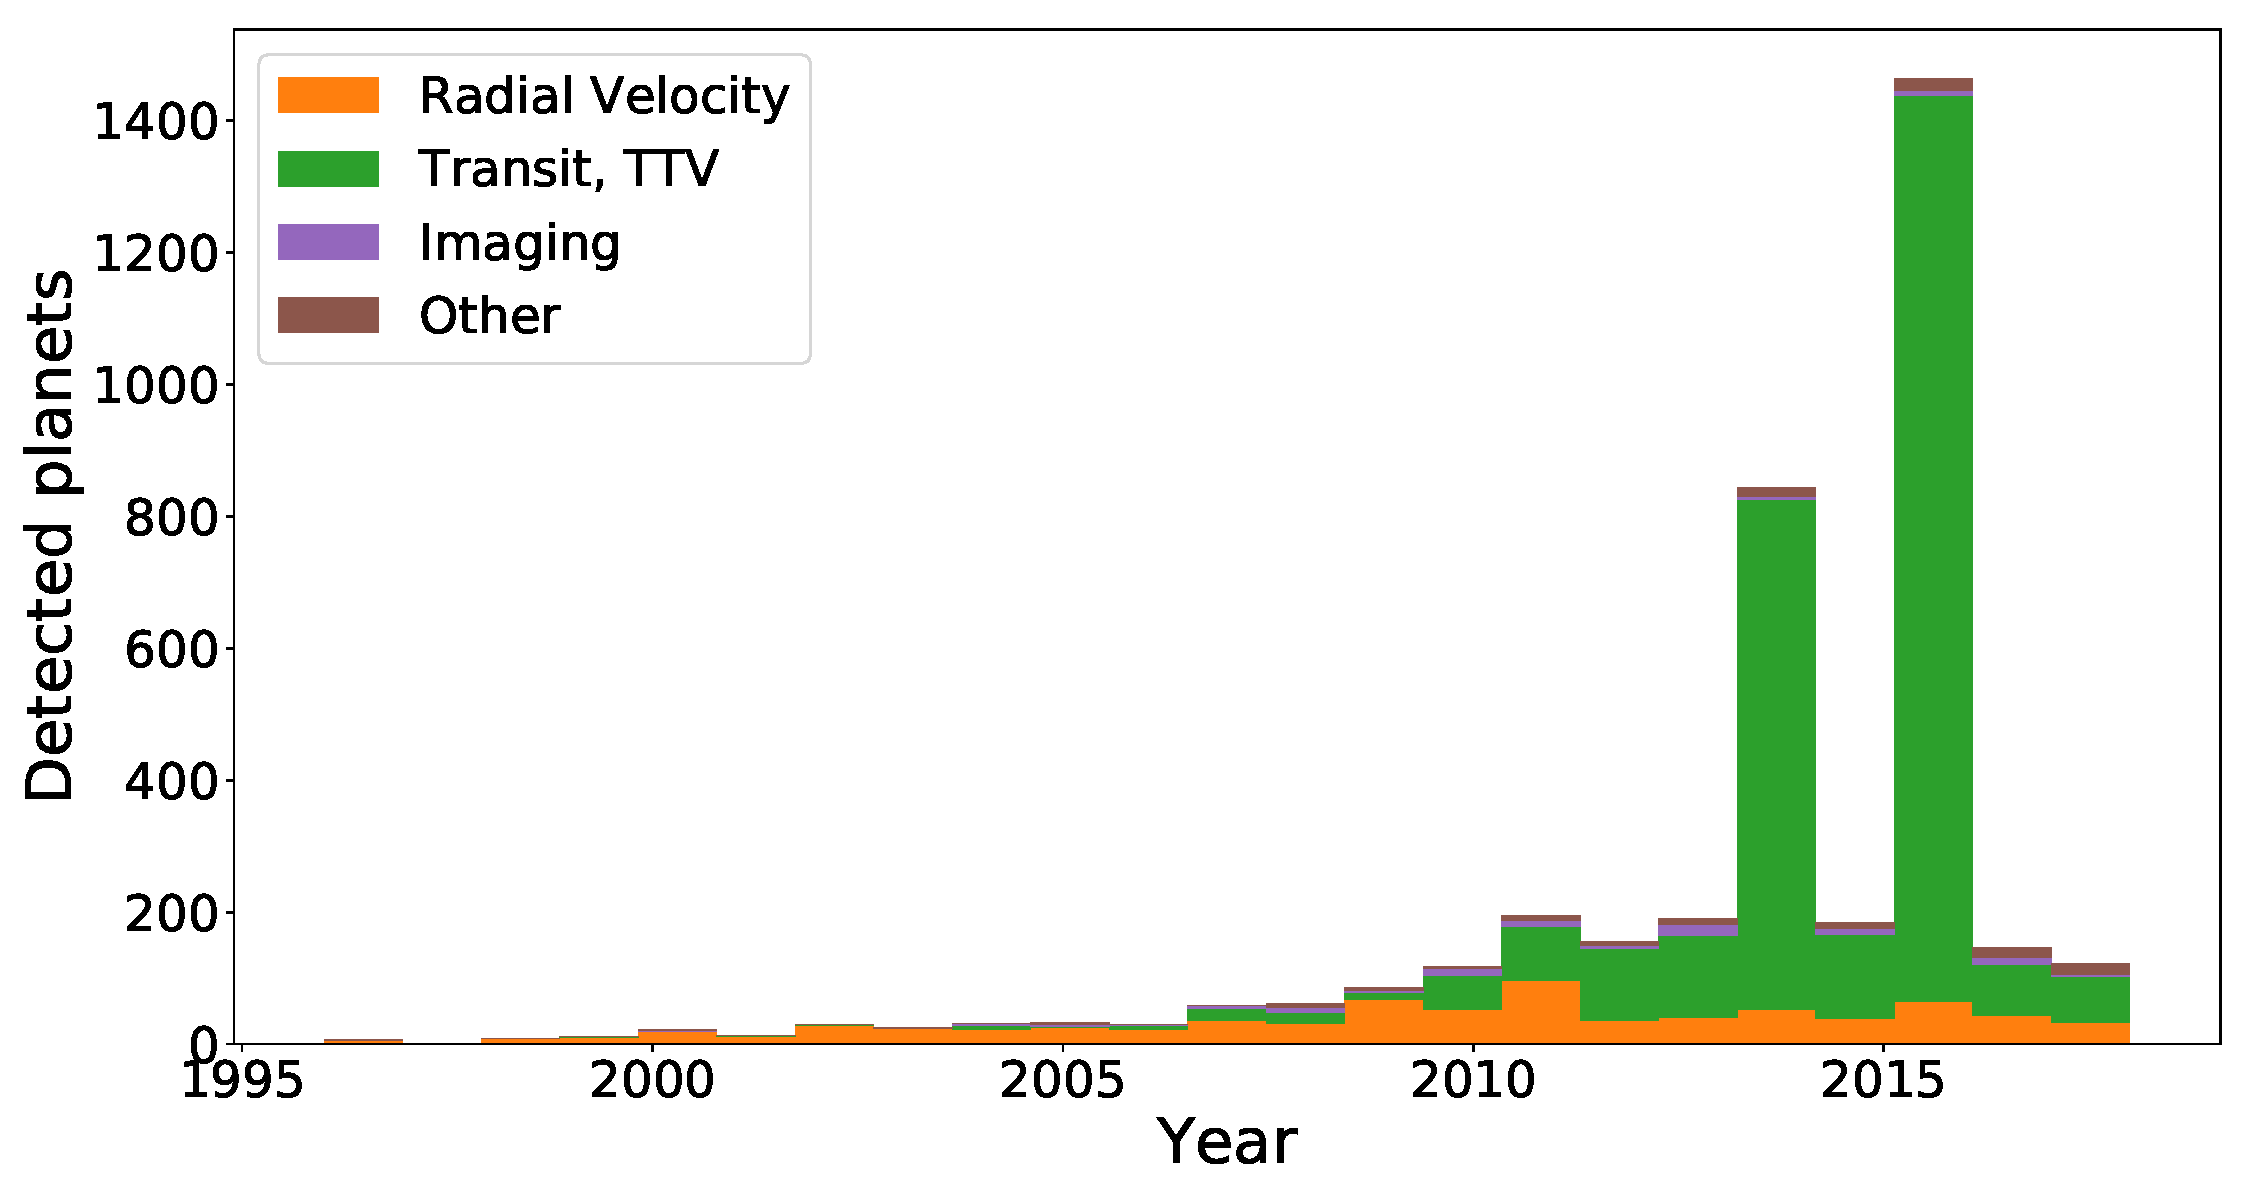
\includegraphics[width=0.7\linewidth]{./figures/introduction/exoplanetEU_year_method.pdf}
    \caption[Number of exoplanet detections per year separated by method.]{Number of exoplanet detections per year separated by method (data from \href{http://ww.exoplanet.eu}{exoplanet.eu} October 2018).}
    \label{fig:detection_year_method}
\end{figure}
\todo{Adjust figure so that can be seen in black and white, textures on bars?}
\subsection{Radial Velocimetry}
\label{subsec:radial_velocimetry}
This technique measures the radial velocity\footnote{Velocity projected along line of sight.} (RV) of the star by analysing the relative Doppler shift of its spectral lines due to the gravitational interaction with a companion.
As the star and companion orbit around their common centre of mass (barycentre) the spectrum of the star periodically oscillates, with the orbital period of the planet, due to the change in relative motion to the observer as depicted in \cref{fig:rvdiagram-mayor} (left).

\begin{figure}
    \centering
    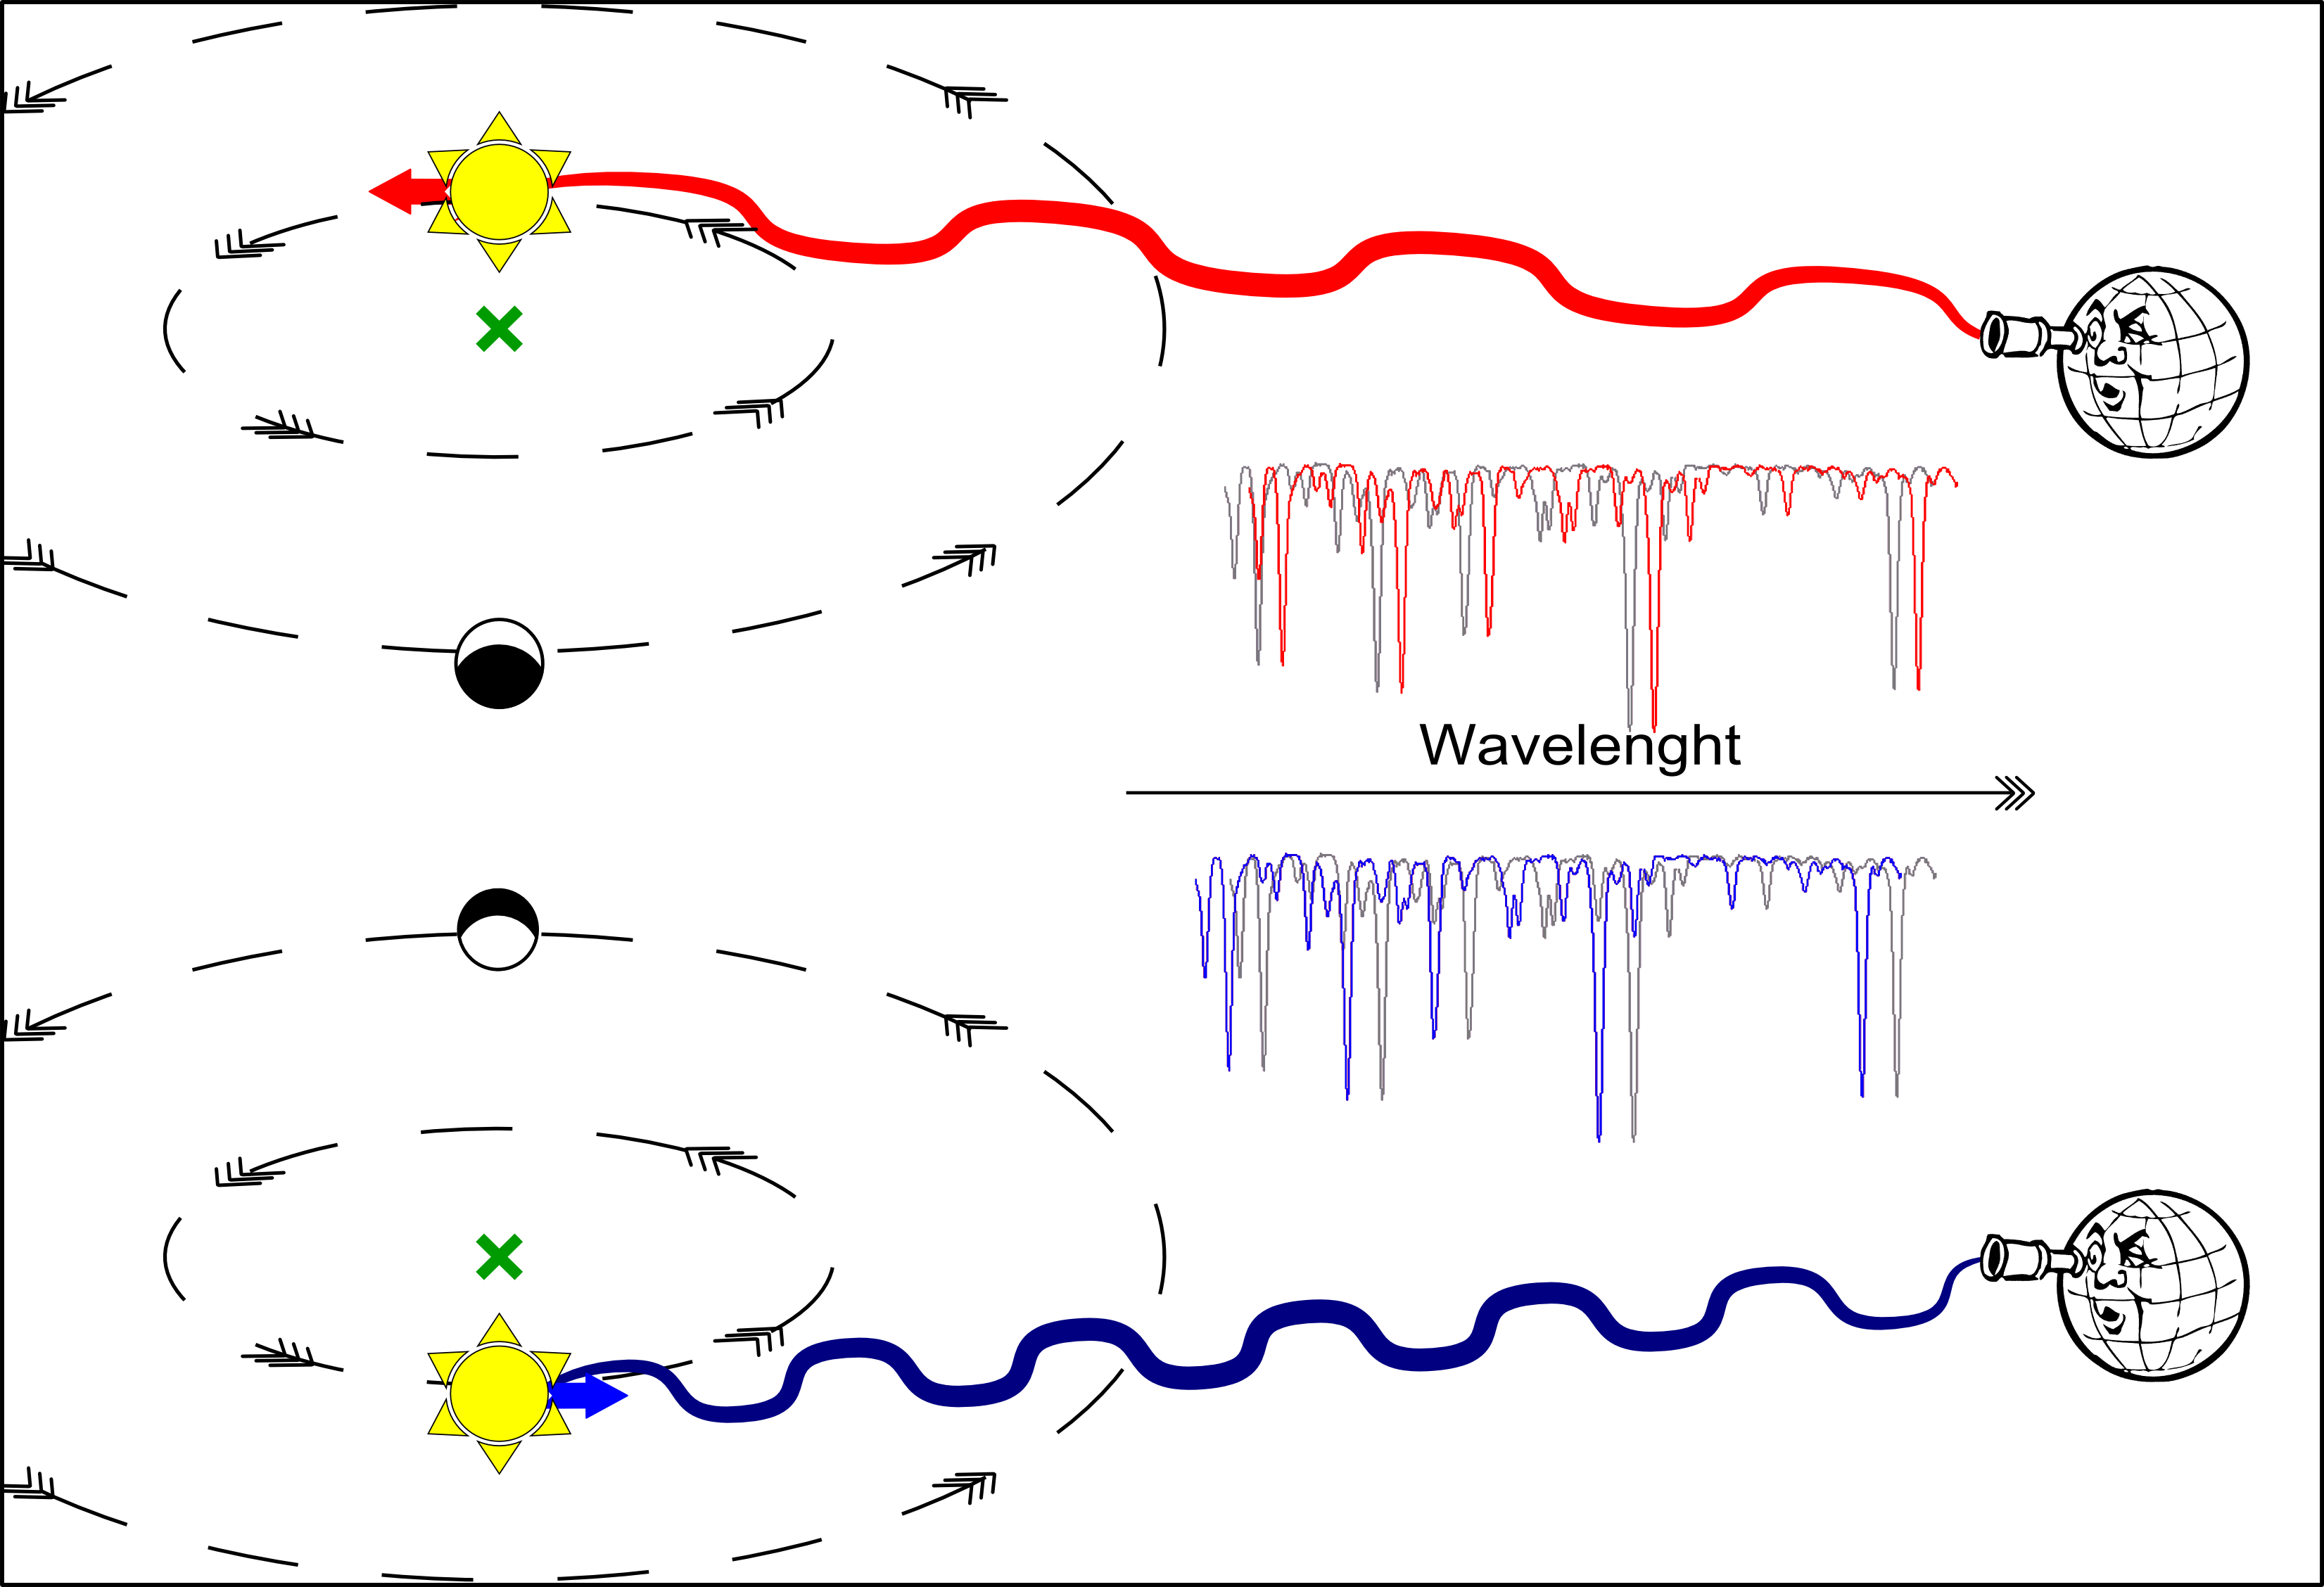
\includegraphics[height=5cm]{./figures/introduction/RV_Diagram}
    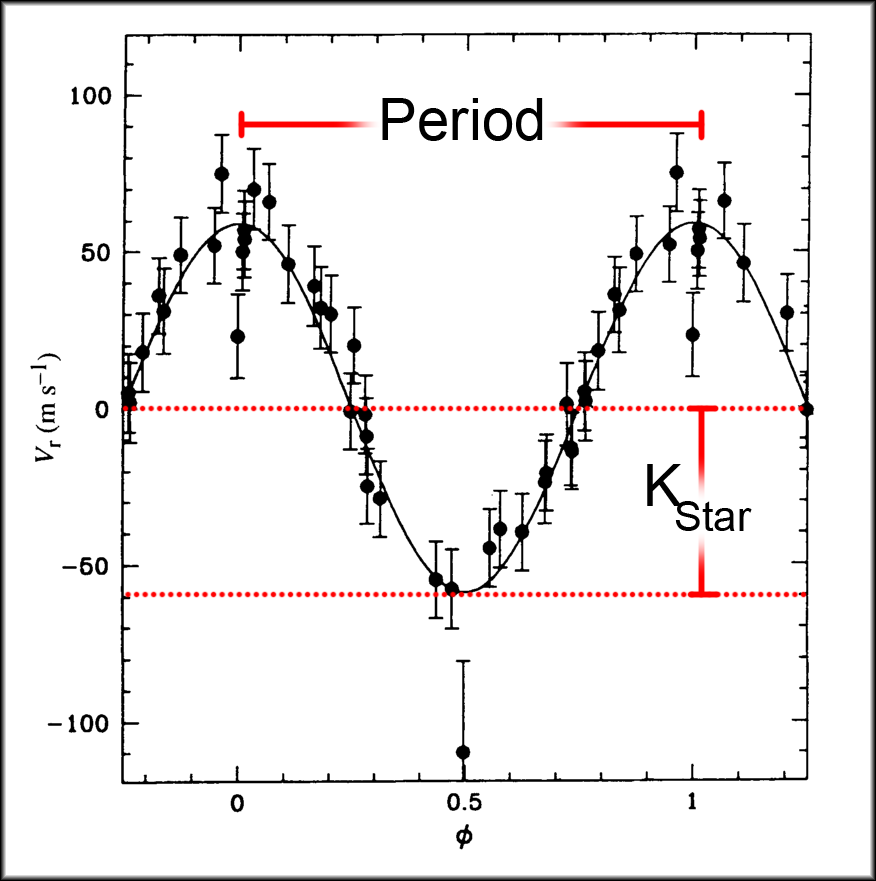
\includegraphics[height=5cm]{./figures/introduction/PhaseFolded_51Pegb_Mayor_et_al_1995}
    \caption[The {RV} method.]{Left: Diagram of {RV} method.
    Right: {RV} variation for the detection of {51 Pegasi}.
    Credit:~\citet{mayor_jupitermass_1995}}.
    \label{fig:rvdiagram-mayor}
\end{figure}

The radial velocity variation, directed along the line of sight, is given by:
\begin{equation}
\label{eqn:rv_equation_intro}
{RV} = \gamma + K [\cos{(\nu(t, P, T_0, e) + \omega)} + e\cos{(\omega)}]
\end{equation}
where \(\gamma\) is constant barycentre velocity of the system relative to the Sun\footnote{Earth's barycentre motion is well known and removed.}, \(K\) is the velocity semi-amplitude, \(e\) the eccentricity, and \(\omega\) is the argument of periastron.
The true anomaly \(\nu\), is a function of time \(t\), orbital period \(P\), and the time of periastron passage \(T_0\), and eccentricity.

The velocity amplitude $K$ of a star of mass $\Mstar$ due to a companion with mass $\Mp$ with orbital period $P$, eccentricity $e$, and inclination\footnote{Relative to a plane that is tangential to the celestial sphere, $i=90$ is edge on.} $i$ is~\citep[e.g.][]{cumming_lick_1999}:
\begin{equation}
    K = {\left(\frac{2\pi G}{P}\right)}^{1/3} \frac{\Mp{} \sin{i}}{{(\Mp{} + \Mstar)}^{2/3}} \frac{1}{\sqrt{1-{e}^{2}}}, \label{eqn:k_amplitude}
\end{equation}
where G is the gravitational constant.

The key exoplanet property determined by the amplitude {RV} technique is the companion mass, relative to the orbital inclination \Mpsini.
As the companion mass is in the numerator of \cref{eqn:k_amplitude} the {RV} technique is more sensitive to larger mass planets.
Also since $K \propto P^{-1/3}$ the amplitude is greater for short period close in orbits\footnote{From Kepler's Law ${P}^{2}\propto {a}^{3}$}.

\begin{figure}
    \centering
    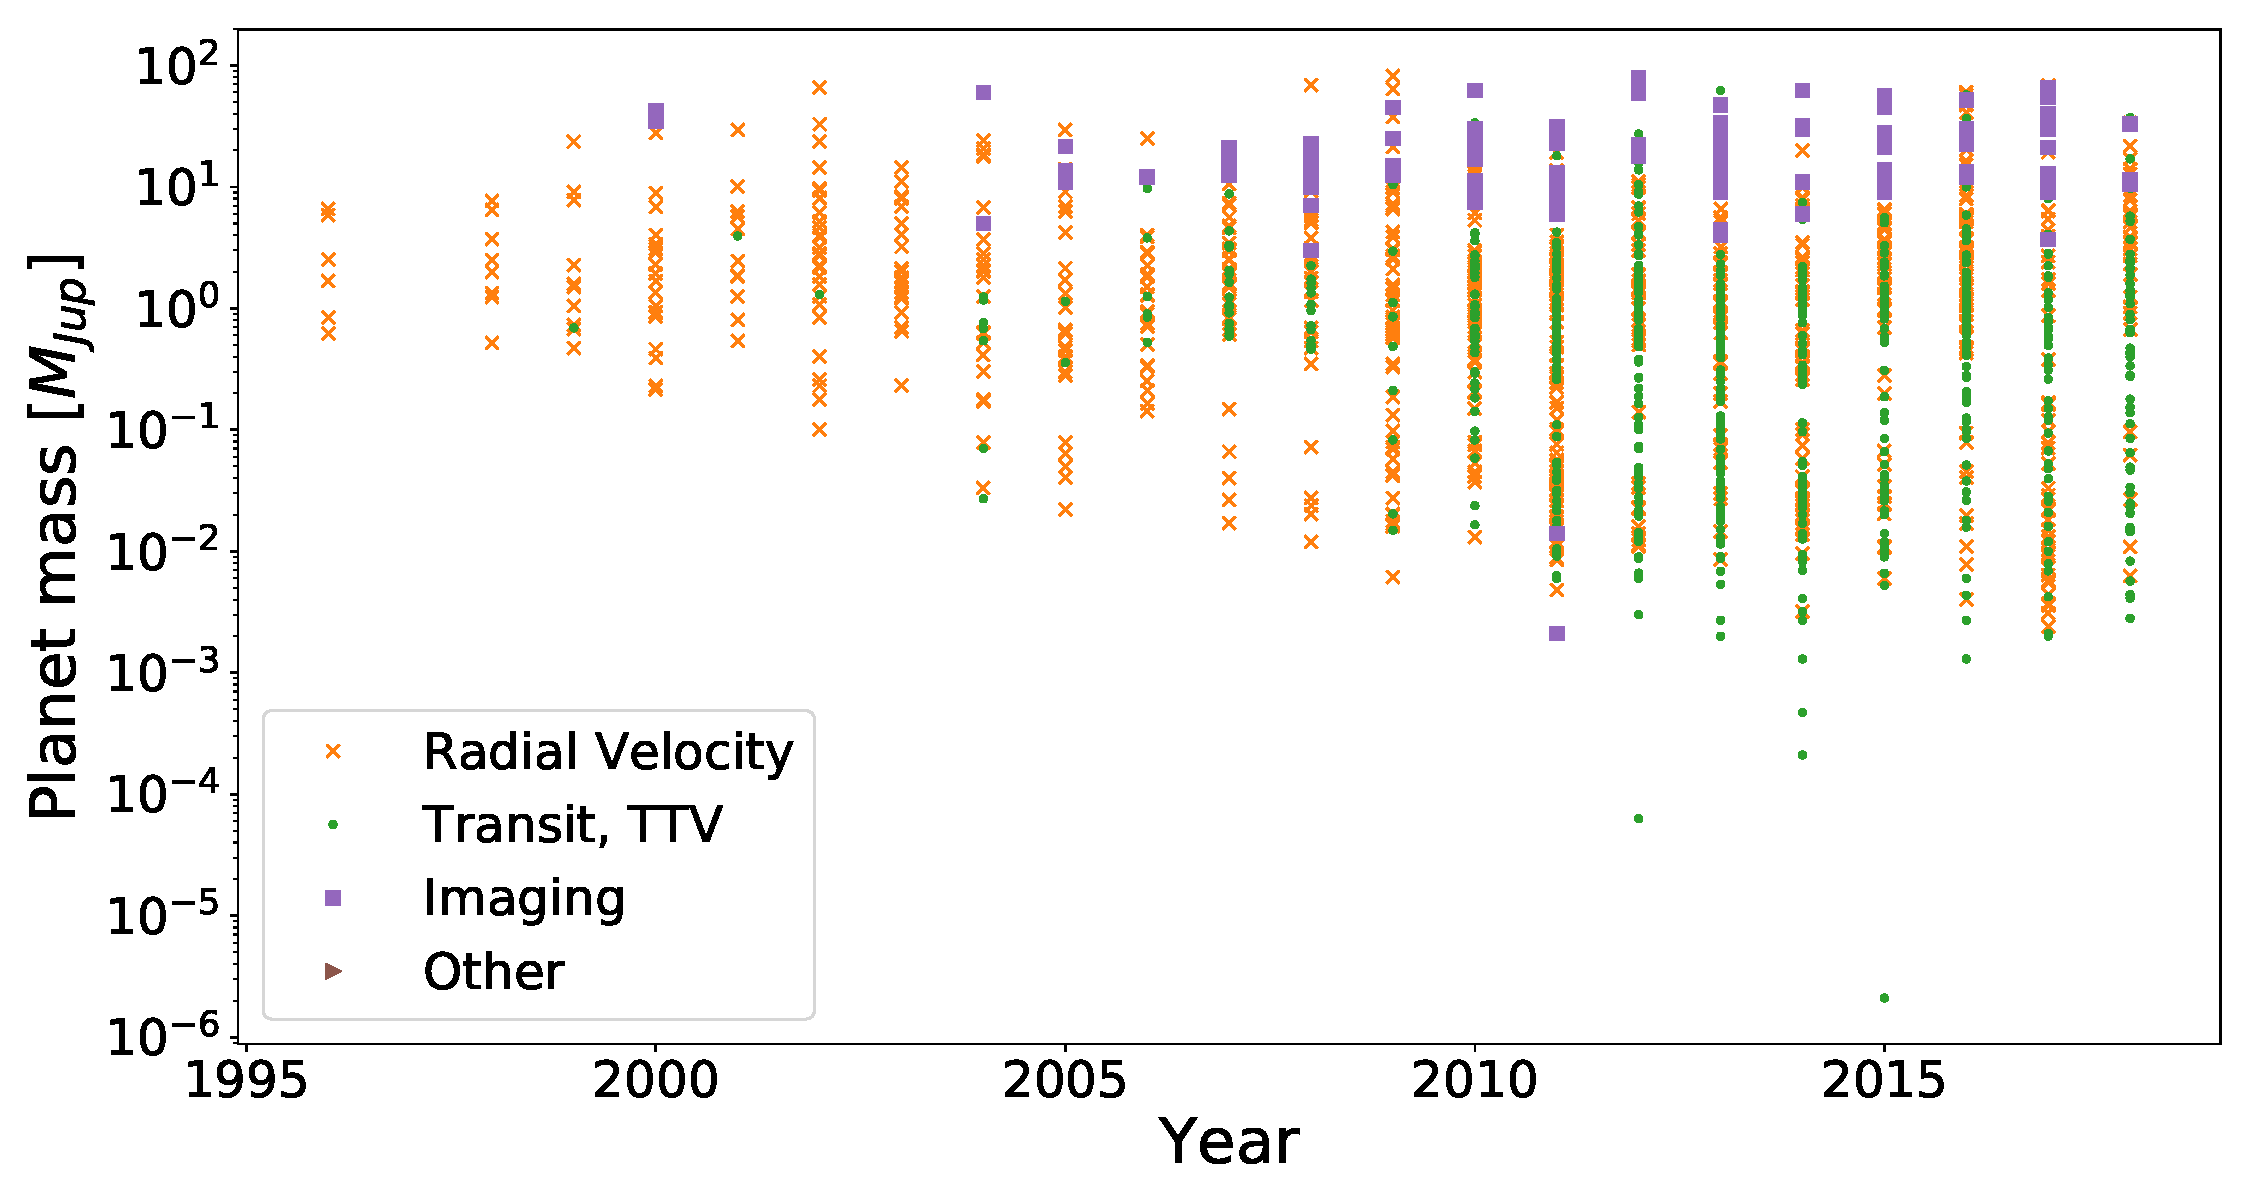
\includegraphics[width=0.7\linewidth]{figures/introduction/exoplanetEU_year_mass.pdf}
    \caption[Exoplanet discovery year verses exoplanet mass.]{Exoplanet discovery year verses exoplanet mass showing a trend towards detecting lower mass planets.
    Exoplanets without a measured mass are not shown.
    The colours indicate the initial detection method.}
    \label{fig:exoplaneteuyearmass}
\end{figure}

The {RV} method kick-started the exoplanet discipline by detecting the first exoplanet around a solar-type star {51 Pegasi}~\citep{mayor_jupitermass_1995}.
The {RV} curve for {51 Pegasi} is shown on the right side of \cref{fig:rvdiagram-mayor}.
The first discoveries were surprising as Jupiter mass planets in short period orbits\footnote{\Mpsini=0.47\,\Mjup{} orbiting at 0.05\AU{} for {51 Pegasi}} were unlike anything in our Solar System and not predicted by standard plant formation theories.
Several exoplanet discoveries followed in quick succession~\citep[e.g.][]{butler_planet_1996, marcy_planetary_1996} with many confirming the existence of the type of planets now referred to as ``hot-Jupiters''~\citep{butler_three_1997, charbonneau_detection_2000}.

The radial velocity amplitudes of the first exoplanets detected were around 60\mps{} while
the radial velocity signal of the Earth in a one year orbit around a solar-type star however is 8.9\cmps{}~\citep[e.g.][]{figueira_radial_2010}.
Dedicated spectrographs, such as HARPS~\citep{mayor_setting_2003} along with improved reduction techniques~\citep{lovis_new_2007} pushed this mass detection limit down to the \mps{} level.
ESPRESSO~\citep{pepe_espresso_2014, megevand_espresso_2014} is the next generation high precision optical spectrograph aiming to push the detection limits to 10\cmps, to detect an Earth twin.
The gradual decrease in measured mass of exoplanets over time is shown in \cref{fig:exoplaneteuyearmass}.
The different symbols indicate the detection method, not necessarily the method used to measure the exoplanet mass.

Most {RV} detection has been performed using optical spectrographs.
However, as the amplitude of {RV} signal is inversely proportional to the mass of the star (RV $\propto \Mstar^{-2/3}$), there are dedicated surveys focusing on smaller mass M-dwarf stars~\citep[e.g.][]{reiners_carmenes_2018}.
M-dwarfs are inherently cooler and thus emit a majority of their stellar output in the near-infrared.
New dedicated high-resolution \nir{} spectrographs have and are being designed and implemented to meet this demand e.g.\ {CARMENES}, {NIRPS}, {SPIRou}, {CRIRES+}.


\subsection{Transit methods}
\label{subsec:transit}
The transit method detects the presence of an exoplanet by observing the periodic dimming of the star due to the passage of the exoplanet between the star and observer, partially blocking the star.
Geometry requires the orbit of the exoplanet to be aligned edge-on to the line of sight (low inclinations) for a transit to occur.
The geometric probability, $P$, that a exoplanet transits is estimated by
\begin{equation}
P \approx \frac{\Rstar}{a (1-{e}^{2})},
\end{equation}
where \(e\) is the eccentricity of the orbit, $\Rstar$ is the star radii and \(a\) is the semi-major axis of the orbit (star-planet distance)~\citep[e.g.][]{barnes_effects_2007}.
The probability of transit increases with the size of the star but decreases with distance to the star.

The drop in stellar brightness during the transit allows the measurement of the planet/star radius ratio:
\begin{equation}
    \frac{\Delta L}{L}\sim{\left(\frac{\Rp}{\Rstar}\right)}^{2}
\end{equation}
where \(L\) is the luminosity of the star, \(\Delta L\) is the maximum luminosity variation (transit depth), and \(\Rstar\) and \(\Rp\) are the radius of the star and planet respectively.

The transit method complements {RV} measurements as the inclination, $i$, of the orbit can be determined from the transit.
This removes the {$\sin{i}$} ambiguity found in the \Mpsini{} of {RV} detections so the true mass, $\Mp$, of the exoplanet can be revealed.
The true mass along with the planet's radius provides a value for the exoplanets average density\footnote{$\rho \equiv \frac{\textrm{Mass}}{\textrm{Volume}} = \frac{3}{4\pi}\frac{\Mp}{\Rp^{3}}$}, hinting at the possible composition.

There are several other astrophysical phenomena which can mimic transiting exoplanet signals, created by configurations of two or more stars which may not involve an exoplanet.
For example a transiting low-mass or white-dwarf star, grazing binary stars, or a transit in a multi-star system~\citep[see e.g.][]{cameron_extrasolar_2012, santerne_contribution_2013}.
Follow-up {RV} observations~\citep[e.g.][]{santerne_radial_2011} are usually required to confirm the planets existence.
Statistical validation techniques are also possible, such as the PASTIS software~\citep{diaz_pastis_2014}, when follow-up can not be performed.
These techniques assess the likelihood of the planet being a true planet against the different false positive scenarios, validating or confirming the planet if the likelihood is high enough.

The transit method has the highest false positive rate among the detection methods presented here.
With {RV} follow-up,~\citet{santerne_sophie_2012} found a false positive rate as high as 35\% for short period giant planets, while~\citet{santerne_sophie_2016} found a 54.6\% false positive rate of 129 giant planets with periods less than 400 days.
These sub-sample false positive rates are however higher than the global false positive rate of 9.4\%~\citep{fressin_false_2013}/11.3\%~\citep{santerne_contribution_2013} found for Kepler.
Some of the currently known exoplanet systems with the smallest radii and lightest mass have been detected through transit and later confirmed with high-precision {RV} follow-up~\citep[e.g.][]{queloz_corot7_2009, pepe_earthsized_2013, lopez-morales_kepler21b_2016, ment_second_2018}.

The identification of unresolved multiple stars, such as a binary or an unrelated background star, can be achieved through high-resolution spectroscopy in which the spectral lines of individual stars can be separated~\citep{kolbl_detection_2015}.
This is important to measure the correct radii of exoplanets as the extra light contribution from an unresolved secondary star will reduce the transit depth, mimicking a smaller transiting planet.

The transit of a single planet can not directly determine the planetary mass.
However, in multiple planet systems, the masses and sometimes the presence of other planets in the system can be determined from perturbations in the transit time and duration~\citep[e.g.][]{holman_use_2005, holman_kepler9_2010}.
A large number of systems have been detected that show transit timing variations (TTV) and transit duration variations (TDV)~\citep[e.g.][]{holczer_transit_2016} due to the gravitational interaction between planets.
The statistical validity of multi-transiting planets is more straightforward than single planets as the probability of having multiple false positives, being the product of the individual probabilities, is lower than having multiple planets in the system~\citep{lissauer_almost_2012}, making multiple planet systems easier to validate.

The presence of star spots on the surface of a star can be observed during transit.
A star spot is a dark region on the stellar surface due to magnetic fields, which decreases the luminosity slightly.
Examples of spots can be seen in the middle of the Sun from an image of the 2012 transit of Venus in \cref{fig:transit_venus_transit_alignment} (left).
It shows several dark sunspots alongside Venus, although Venus did not cross them.
Unlike for other stars, sunspots are spatially resolved.
If an exoplanet passes in front of a spot, the luminosity decrease from the spot is temporarily hidden and a small bump occurs in the transit shape.
The presence of spots in successive transits (see \cref{fig:transit_venus_transit_alignment} (right)) can indicate the alignment of the stellar rotation to the planet orbital plane~\citep{sanchis-ojeda_starspots_2013}.
In this simulation an orbit aligned with the stellar rotation and the transit crosses the spot in four successive orbits.
In a misaligned case a spot would only be observed in one transit.

\begin{figure}
    \centering
    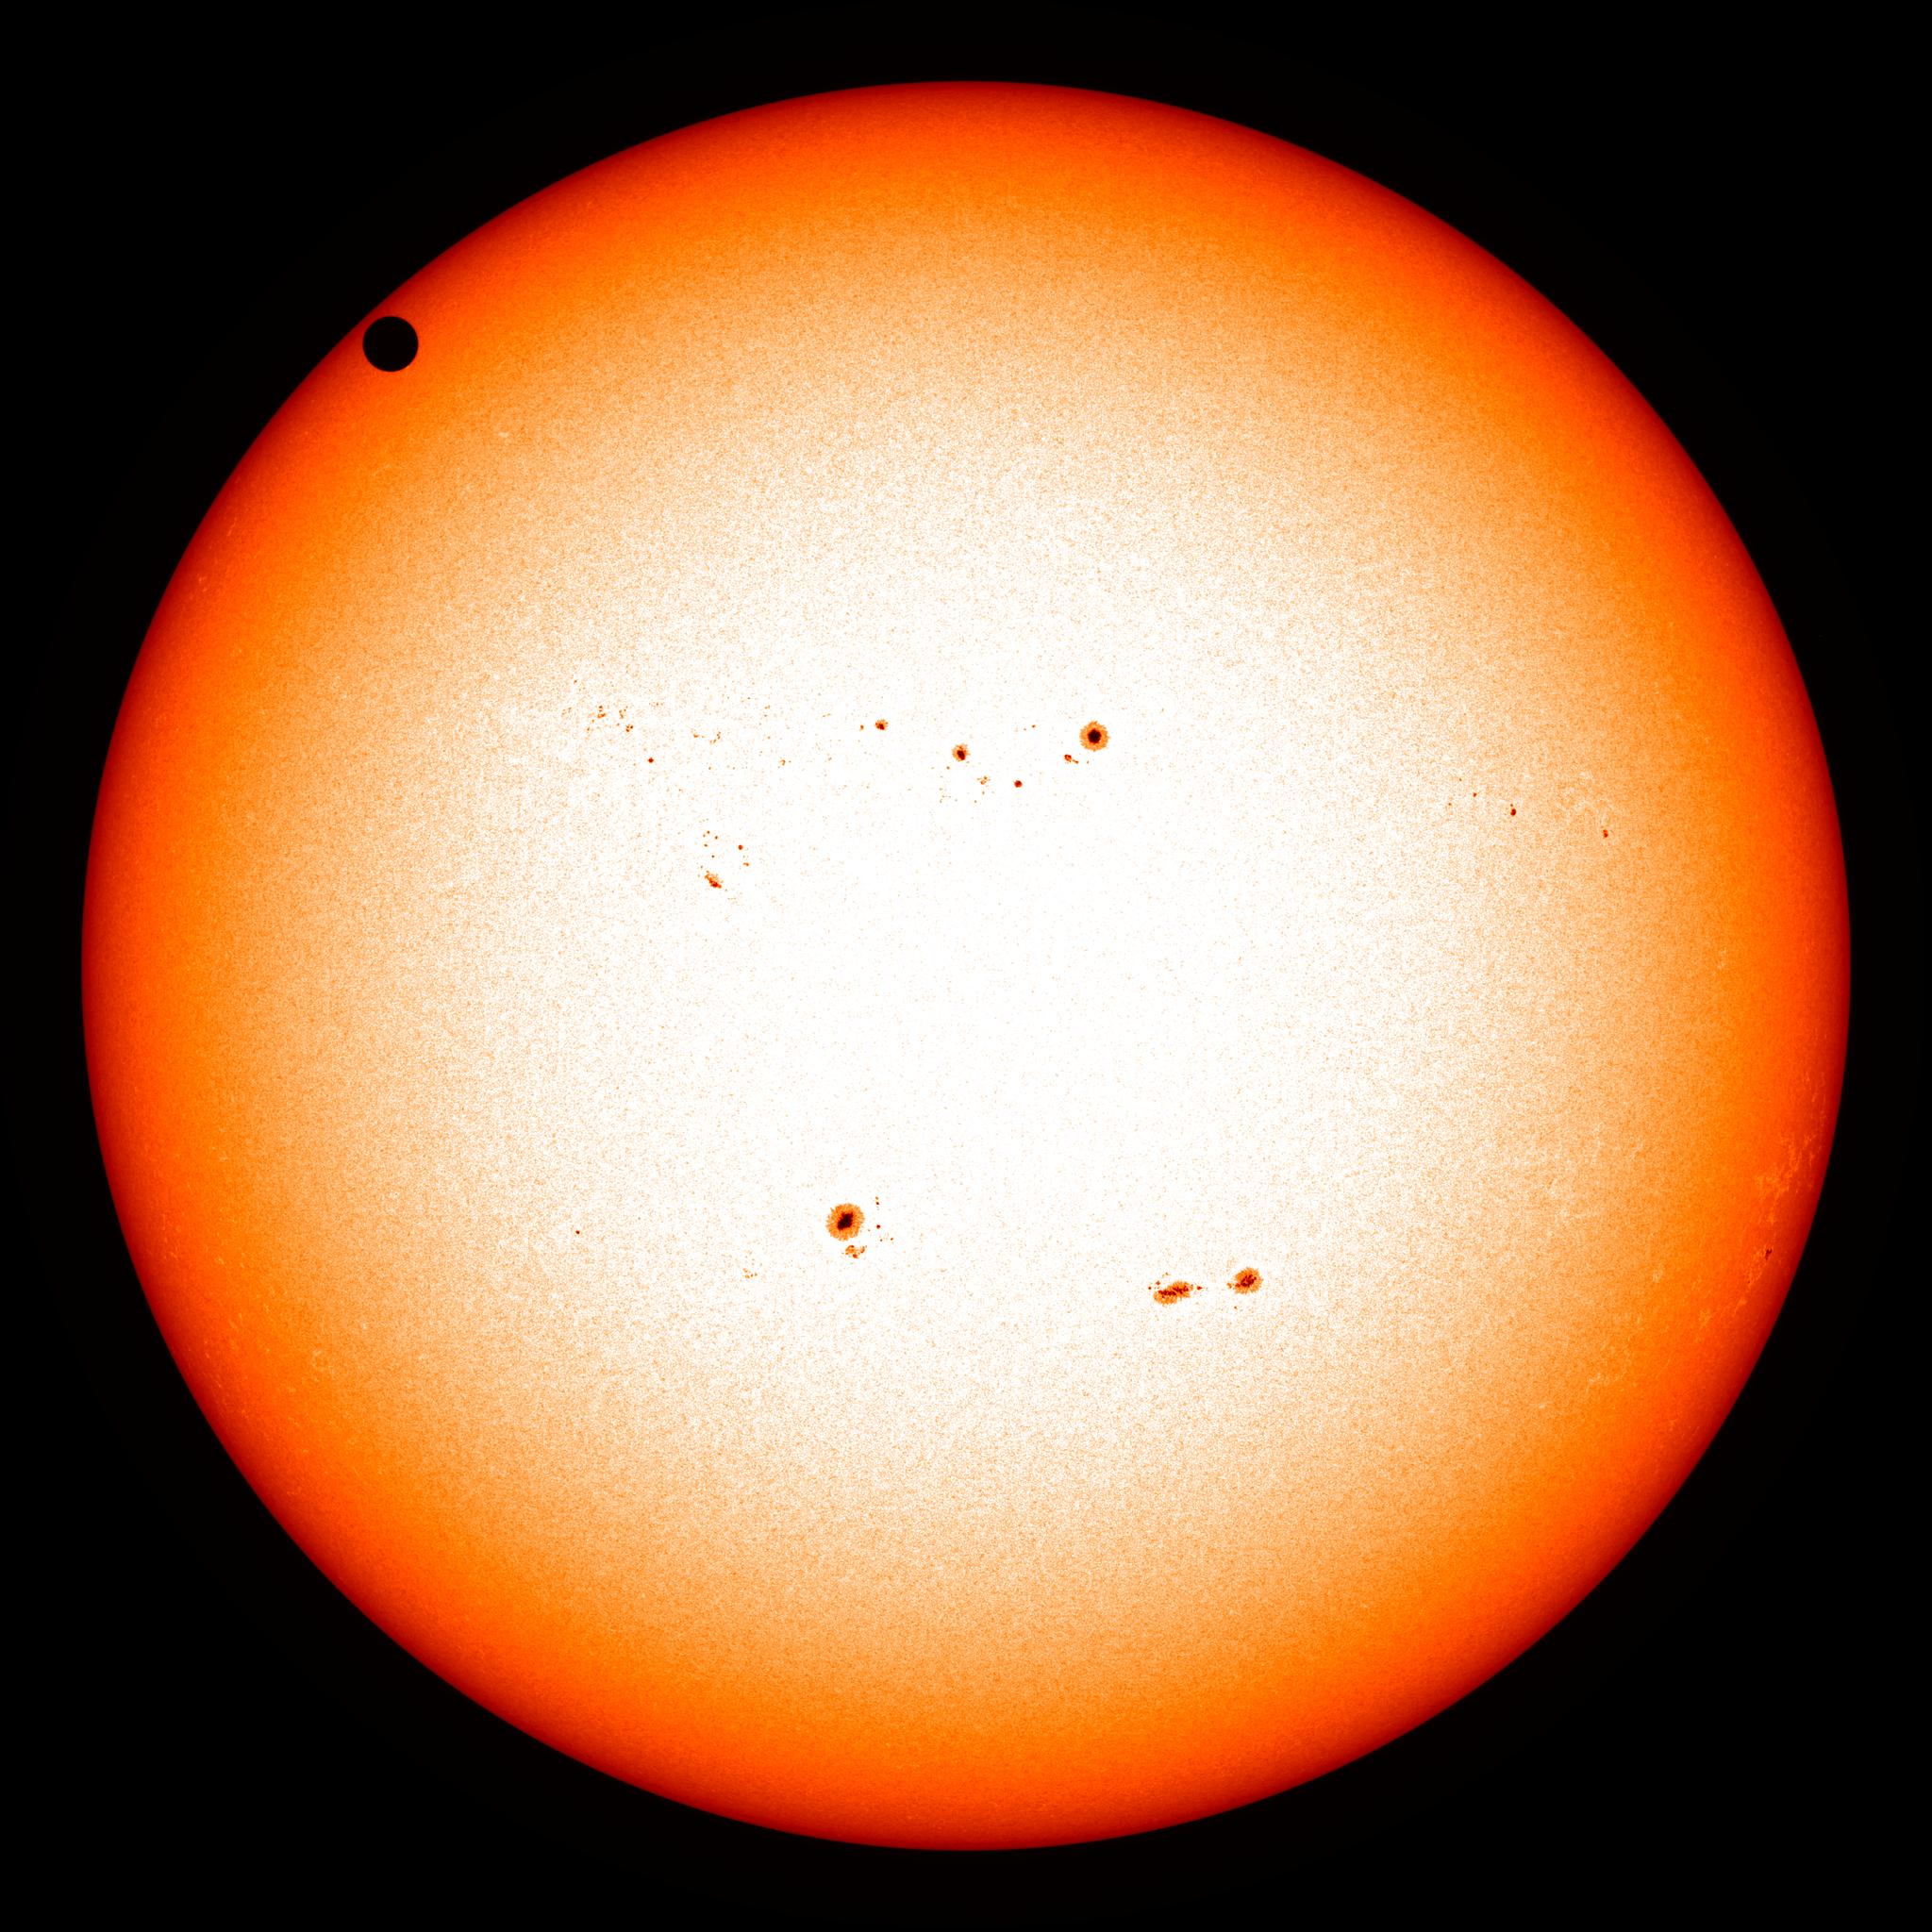
\includegraphics[height=5cm]{./figures/introduction/SDO_2012_Venus_Transit.jpg}
    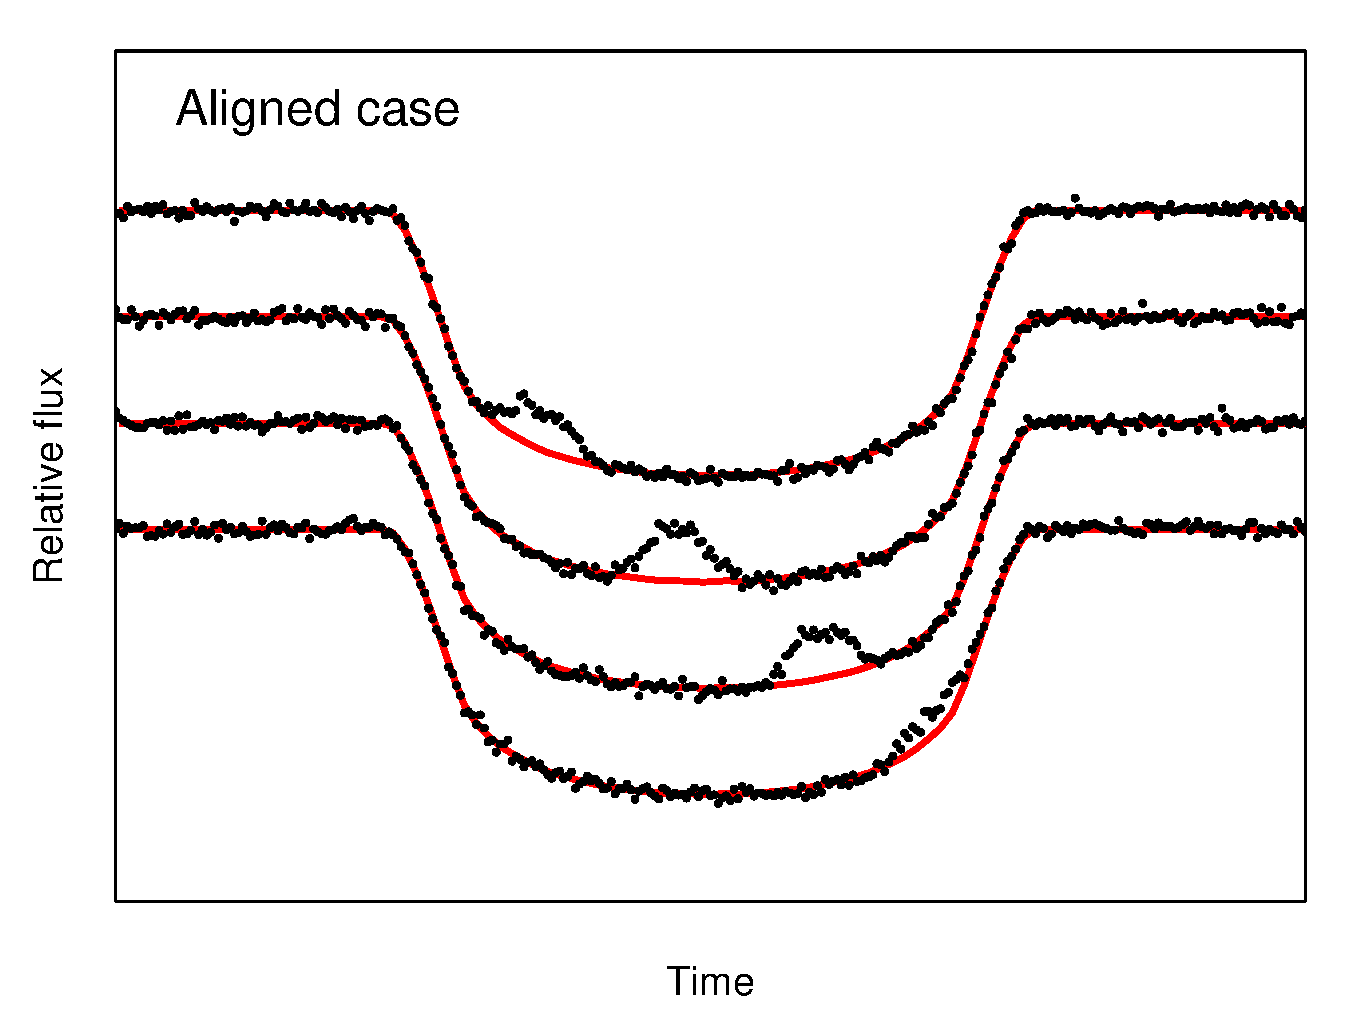
\includegraphics[height=5cm]{figures/introduction/sanchisojedafig1-crop.pdf}
    \caption[Transit of Venus and successive transit corssings.]{Left: Image from the 2012 transit of Venus obtained from the Solar Dynamics Observatory satellite.
    Venus is the dark circle in the top left of the Sun.
    Limb darkening is observed as the change in colour/brightness from white to red near the edge.
    Several sunspots are also observed on the surface of the Sun.
    Credit: {NASA}/{SDO}, {HMIR}.
    Right: Simulation of 4 successive transits crossing a star spot with the orbit aligned with the stellar rotation.
    The stellar rotation is 1/10 the orbital period.
    Adapted from~\citet[][Figure~1]{sanchis-ojeda_starspots_2013}.}
    \label{fig:transit_venus_transit_alignment}
\end{figure}


The vast majority of transit detections have come from Kepler~\citep{borucki_characteristics_2011}, which focused on a small patch of sky (0.25\%) for four years continuously.
Kepler's impressive sensitivity compared to previous surveys, allowed it to detect planets down to around 2\Rearth.
However, {CoRoT}~\citep{barge_transiting_2008} and ground-based surveys, such as WASP~\citep{pollacco_wasp_2006}, OGLE~\citep{udalski_optical_2002}, TreS~\citep{alonso_tres1_2004} have also had successful transit detections.

Following in Kepler's footsteps the next generation transit hunter {TESS}~\citep{ricker_transiting_2015} has already announced discoveries of new transiting planets only months after launch~\citep{vanderspek_tess_2018, gandolfi_tess_2018, huang_tess_2018}.
It will eventually cover more than 90\% of the sky with an impressive planetary yield expected of $\sim10\,000$ exoplanets, with around 3500 the size of Neptune or smaller~\citep{barclay_revised_2018, huang_expected_2018}.
However, the observation coverage is not uniform, with the majority of the ecliptic plane receiving only one month of observations, limiting the detection sensitivity to short period transiting planets.
On the other hand, the ecliptic poles will receive almost one year continuous observation.

{PLATO} \citep{rauer_the_2014} is another transit survey mission planned for launch in 2026.
In contrast to Kepler it will focus on brighter nearby, stars, with the goal to detect and accurately determine the planetary parameters of Earth-like planets in the habitable zone.

A smaller transiting mission, {CHEOPS} \citep{broeg_cheops_2013}, is also scheduled for launch at the end of 2019.
Unlike the transiting surveys mentioned above, {CHEOPS} will perform dedicated transit follow-up of bright stars with known planets, such as those found with {RV} surveys.
It will providing high precision transit photometry, if the geometry allows, to obtain precise planetary radii.


\subsection{Direct Imaging}
\label{subsec:direct_detection}
The direct imaging technique involves directly imaging an exoplanet in orbit around a star.
The first planets directly imaged were {2MASSWJ~1207334--393254~b} using adaptive optics with NACO on the VLT~\citep{chauvin_giant_2004}, three planets around HR\,8799 using angular differential imaging on the Keck and Gemini telescopes~\citep{marois_direct_2008}, and {Fomalhaut~b} using chronography on the HST~\citep{kalas_optical_2008}.
As an example, the direct image of {HR\,8799} is shown in \cref{fig:directimaging}, where a fourth planet was revealed~\citep{marois_images_2010}.

Direct imaging requires resolving the angular separation between the star and planet and is best suited to detect giant planets in wide orbits (>10\AU{}) around nearby stars.
This is shown by the clustering of direct image detections shown in \cref{fig:exoplaneteuyearmass}.
Extremely young giants observed in the infrared are favoured as they have higher thermal emissions (while they are still cooling) and larger surface area resulting in a higher contrast ratio to the host.


\begin{figure}
    \centering
    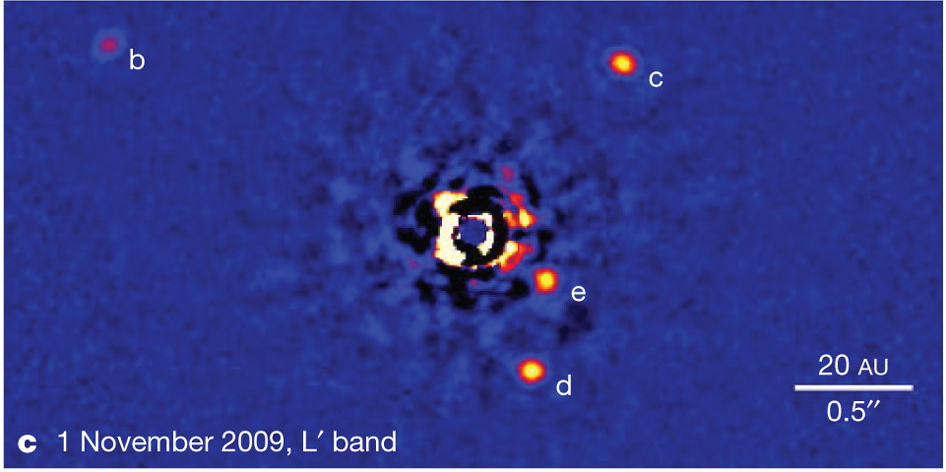
\includegraphics[width=0.5\linewidth]{./figures/introduction/DirectImaging_HR8799_MaroisEtAl2010}
    \caption[Direct detection of four exoplanets around HR\,8799.]{Direct detection of four exoplanets around HR\,8799~\citep{marois_images_2010}.}
    \label{fig:directimaging}
\end{figure}

High-contrast adaptive optics instruments, such as SPHERE@VLT~\citep{beuzit_sphere_2008} and GPI~\citep{macintosh_gemini_2008}, are being used with several different techniques to observe targets closer to the star and with smaller contrasts, usually involving blocking or cancelling out the light from the star while retaining the signal of the planet~\citep[e.g.][]{marois_direct_2005, mawet_annular_2005, schmid_zimpol_2005, sirbu_prospects_2017, sirbu_techniques_2017, wang_observing_2017}.
Ground based direct imaging requires adaptive optics to reduce the turbulence induced by the atmosphere, increasing the angular resolution down to the telescope diffraction limit.

On top of hardware based solution to the stellar contamination, cleaver observing strategies and cancelling algorithms.
Angular differential imaging (ADI) \citep[eg.][]{marois_direct_2005} is one such technique.
ADI, disables the field de-rotator component in the telescope so that the viewing field rotates relative to the plane of the detector during the night.
Several images taken at different angles are rotated to a reference position and stacked.
The stacking of images from different angles cancels out the pseudo-static speckle caused by the telescope and optics while increasing the contrast of any faint object in the stars vicinity, i.e. a planetary companion.

The direct imaging technique is also used to observe circumstellar and protoplanetary disks, and has even captured images of planets during formation~\citep[e.g.][]{sallum_accreting_2015}.
Combining direct images from different photometric bands can allow for the creation of low-resolution exoplanet spectra~\citep[e.g.][]{kuzuhara_direct_2013, zurlo_new_2015}.


\subsection{Astrometry}

\label{subsec:astrometry}
Astrometry measures the precise position of the stars on the plane of the sky.
The motion of a star with an exoplanet about its centre of mass can be observed in the periodic oscillating of position from its proper motion in the sky.

For a circular orbit the angle of the semi-major axis of the apparent orbital ellipse, the amplitude of the astrometric signature ($\theta$), is given by
\begin{equation}
\theta = \frac{M_{p}}{M_{star} + M_{p}} \frac{a}{d}
\end{equation}
where, $\Mp$ and $\Mstar$ are the planet and stellar mass, $a$ is the semi-major axis (in \AU) and $d$ is the distance from the observer to the system (in parsec)~\citep{perryman_exoplanet_2011}.

This shows that the astrometric signal is proportional to the companion/star mass ratio and to the orbital radius, $a$.
The amplitude also decreases inversely with distance, as the angles become smaller.
This is unlike the {RV} and transit methods for which the amplitude is not affected by distance.
Astrometry is complementary to the {RV} method as it measures the orbital motion perpendicularly to the line of sight, allowing the three-dimensional orbit to be determined.

A modelled astrometric signal is shown in \cref{fig:astrometry_perryman}, for a star at a distance of 50\pc, with a proper motion of 50\masperyr{}, and orbited by a planet of $\Mp = 15$\,\Mjup{}, $e = 0.2$, and $a = 0.6$\AU~\citep{perryman_extrasolar_2000}.
The straight dashed line shows the path of the system's barycentric motion viewed from the Solar System barycentre.
The dotted line shows the effect of parallax (the Earth's orbital motion around the Sun, with a period of 1 year).
The solid line shows the apparent motion of the star as a result of the planet, the additional perturbation being magnified by $\times 30$ for visibility.

Although astrometry has detected many binary stars~\citep[e.g.][]{gontcharov_new_2000} and found several brown-dwarf companions~\citep[e.g.][]{sahlmann_search_2011}, the exoplanet discovery's are few.
A 1.5\,\Mjup{} mass planet in a roughly 1000 day orbit around {HD\,176051} was reported by~\citet{muterspaugh_phases_2010}, and recently the astrometric perturbation of a known planet, {Beta Pictoris~b}, was performed utilizing measurements from {GAIA}~\citep{collaboration_gaia_2016a} and {HIPPARCOS}~\citep{esa_hipparcos_1997} to determine a mass of 11\,\Mjup~\citep{snellen_mass_2018}.

The predicted astrometric variations for an exoplanet are at the level of sub-milliarcseconds and therefore are not achievable from the ground due to atmospheric turbulence.
The most precise astrometric measurements come from spacecraft.
These are currently being performed using GAIA with the recent release of astrometric parameters for 1332~million sources~\citep{collaboration_gaia_2018} and reaching a precision of 0.04\,mas for the brightest stars (<14 magnitude).
Simulations predict that more than 21\,000 large mass planets (1--15\,\Mjup) in long-period orbits should be discovered during the 5 year nominal GAIA mission~\citep{perryman_astrometric_2014}.

\begin{figure}
    \centering
    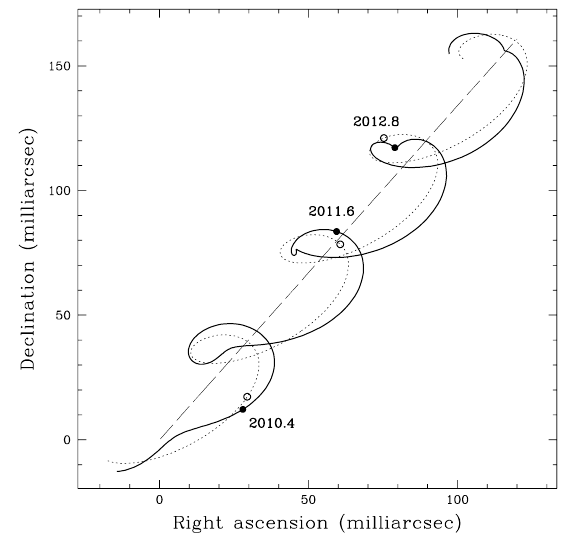
\includegraphics[width=0.5\linewidth]{./figures/introduction/Astrometry_Perryman2000.png}
    \caption[Modelled astrometric path on the sky.]{The modelled astrometric path on the sky from~\citet{perryman_extrasolar_2000}.
    Showing a star at a distance of 50\pc, with a proper motion of 50\masperyr{}, and orbited by a planet of $\Mp$ = 15\,\Mjup{}, $e$ = 0.2, and $a$ = 0.6\AU{}.
    The straight dashed line shows the path of the system's barycentric motion viewed from the Solar System barycentre.
    The dotted line shows the effect of parallax (the Earth's orbital motion around the Sun, with a period of 1 year).
    The solid line shows the apparent motion of the star as a result of the planet, the additional perturbation being magnified by $\times 30$ for visibility.}
    \label{fig:astrometry_perryman}
\end{figure}


\subsection{Microlensing}
\label{subsec:microlensing}
Microlensing is an astronomical effect predicted by Einstein's General Theory of Relativity.
The mass of an object bends space-time which causes light to be visibly deflected around large mass objects.
As a star passes between Earth and a distant star it acts like a lens, bending and magnifying the light from the background star.
The gravitation of a planet orbiting the lens star (if it exists) creates a distortion in the lens, leading to small caustics, deviations in the microlensing light curve for a single lens event (star without a planet).

An example is shown in \cref{fig:microlensing_example} where a lensing magnification of up to $\times3$ is observed for {OGLE2005-BLG-390}~\citep{beaulieu_discovery_2006}.
On the falling edge of the lensing event (and inset top right) there is a bump due to the presence of a 5.5\,\Mjup{} companion.

The difficulties of microlensing is that they require the chance alignment between Earth, a nearby lens star, and a distance source star, which is unrepeatable.
Some caustics are often difficult to fit and yield degenerate results, making characterization of the planet difficult.
Follow-up measurements of a handful of microlensing events have been performed~\citep[e.g.][]{kubas_frozen_2012, batista_confirmation_2015, santerne_spectroscopic_2016} to break degeneracies.
However, follow-up can be difficult as microlensing is sensitive to distant host stars, which are outside the ability of current spectrographs.
It is also sensitive to planets with a wider orbital separation compared to transits and {RV}.
Currently there are 87 planets in 82 systems detected by microlensing, as listed in the \href{https:\\www.exoplanet.eu}{exoplanet.eu} database.

The microlensing technique has been efficient in detecting Neptune analogue planets, distant planets similar in size to Neptune.
Showing that cold Neptune planets are likely most common pe of planet outside of the snow line \citep{suzuki_exoplanet_2016}, the distance from the star at which point it is cold enough for volatile compounds (e.g.\ \ce{H20}, \ce{NH3}, \ce{CO2}) to condense into solid ice grains.

Microlensing events are detected and monitored using dedicated global telescope networks such as {OGLE}, {MOA}, {microFUN} and {PLANET}.
They focus their viewing towards the galactic bulge where there are more stars and a higher chance for microlensing events to occur.

The precise stellar proper motions from the GAIA mission are being used to predict possible future alignments that could produce microlensing events~\citep{kluter_prediction_2018}

\begin{figure}
    \centering
    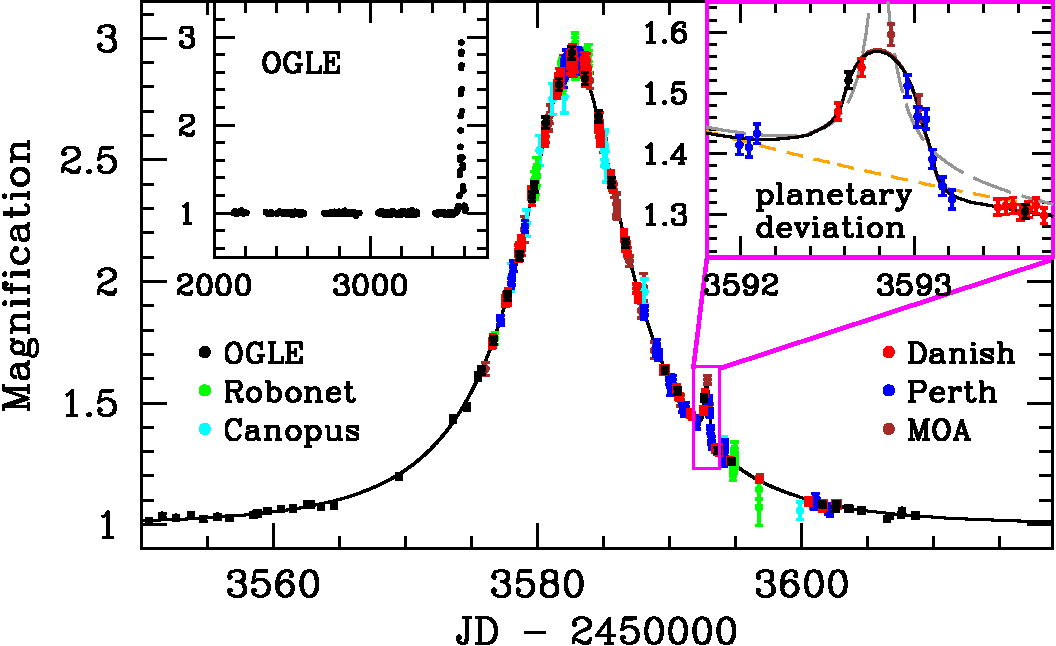
\includegraphics[width=0.5\linewidth]{./figures/introduction/Microlensing_OGLE2005-BLG-390.pdf}
    \caption[Microlensing magnification of OGLE2005-BLG-390.]{Microlensing magnification of OGLE2005-BLG-390 from~\citep{beaulieu_discovery_2006}.
    The presence of the 5.5\,\Mjup{} planet causes the small bump shown in the upper right inset plot.}
    \label{fig:microlensing_example}
\end{figure}

\subsection{Pulsar timing}
\label{subsec:pulsar_timing}
Pulsars are rapidly rotating neutron stars or white dwarfs formed after the death of a giant star, that radiate an intense electromagnetic beam.
The timing variations of the millisecond pulsar\footnote{Rotating at 9\,650 revolutions per minute} {PSR1257+12} led to the first extrasolar planet detection~\citep{wolszczan_planetary_1992}.
There are two models of planet formation around pulsars: either they formed before the supernova explosion and survived, or they formed after, from the remnants of the supernova~\citep{starovoit_existence_2017}.
There is still a rarity of less than 10 pulsars with known orbiting planets.

The rarity of these events is partially associated to the technique which requires very precise instrumentation on high cadence (< milliseconds) to precisely measure the electromagnetic radiation from the pulsar.
For example the first pulsar was detected with the Arecibo radio telescope.
With the primary dish fixed into the mountain, its pointing is limited and achieved by moving the receiver.
It has a limited number of stars that can be observed with a sufficient time coverage to detect planets around pulsars.



%!TEX root = ../../thesis.tex

\section{Detecting atmospheres}
\label{sec:decting_atmopsheres}
To help characterize an exoplanet, a detection of its atmosphere can provide useful information.
After the detection of exoplanets and the measurement of their bulk properties, detecting their atmospheres is the next step.
The detection of planetary atmosphere is difficult due to the low planet-to-star flux ratio.
This requires high precision instrumentation to detect.
For example the planet-to-star flux ratio in the optical is $\approx 10^{-4}$ for a hot Jupiter with a 3 day orbit, in which the main component is reflected star light.
In the infrared the thermal emission of the planet dominates and the flux ratio rises to $\approx 10^{-3}$.
These flux ratios requires observations with signal-to-noise ratios of $10^4$ and $10^3$ in the optical and infrared respectively to achieve a planetary signal at the same level as the noise level.
These detections are only just at the capabilities of the current generation of technology, and with very long observation cost.

Several photometric and high-resolution spectroscopic techniques are showing promising results; these are detailed in the following sections.


\subsection{Occultation and phase variations}
\label{subsec:phase_variation}

\begin{figure}
    \centering
    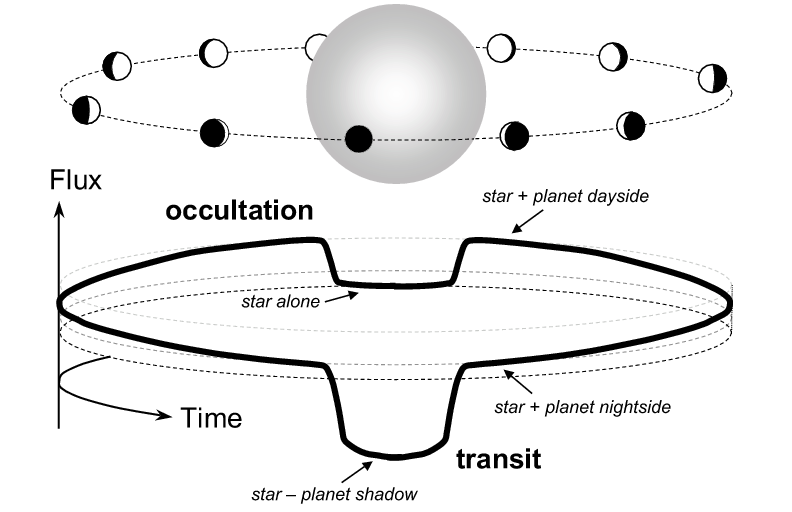
\includegraphics[width=0.6\linewidth]{./figures/introduction/circular_diagram.png}
    \caption[Flux contribution from a star and planet in a transiting exoplanet system.]{Illustration of the flux contribution from a star and planet in a transiting exoplanet system throughout its orbit.
        Credit~\citet{winn_transits_2010}.}
    \label{fig:transits_and_occultations}
\end{figure}

\begin{figure}
    \centering
    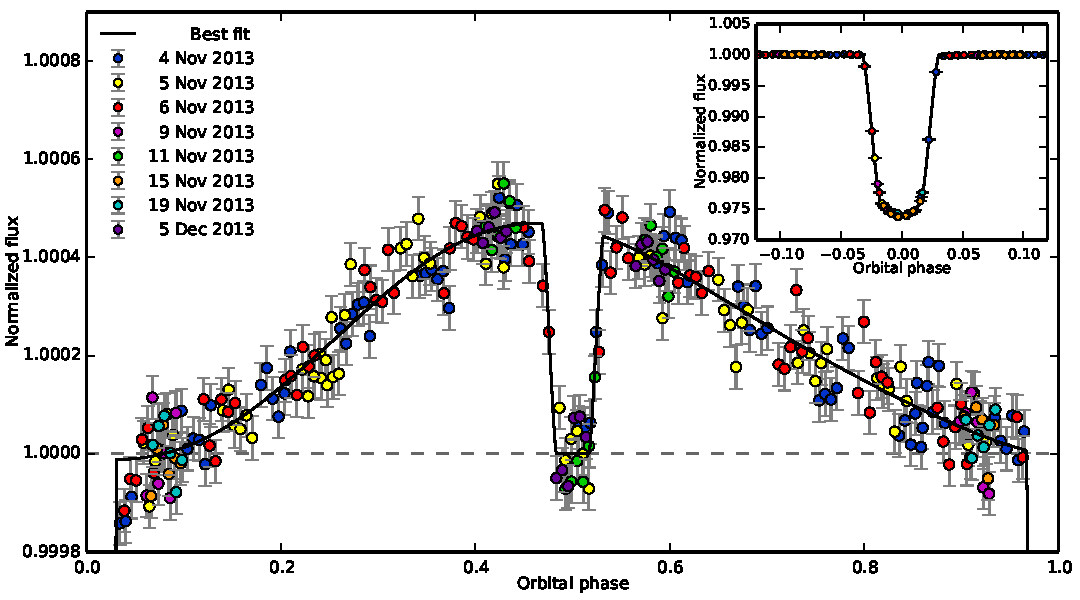
\includegraphics[width=0.5\linewidth]{figures/introduction/stevenson_phasecurve2014.pdf}
    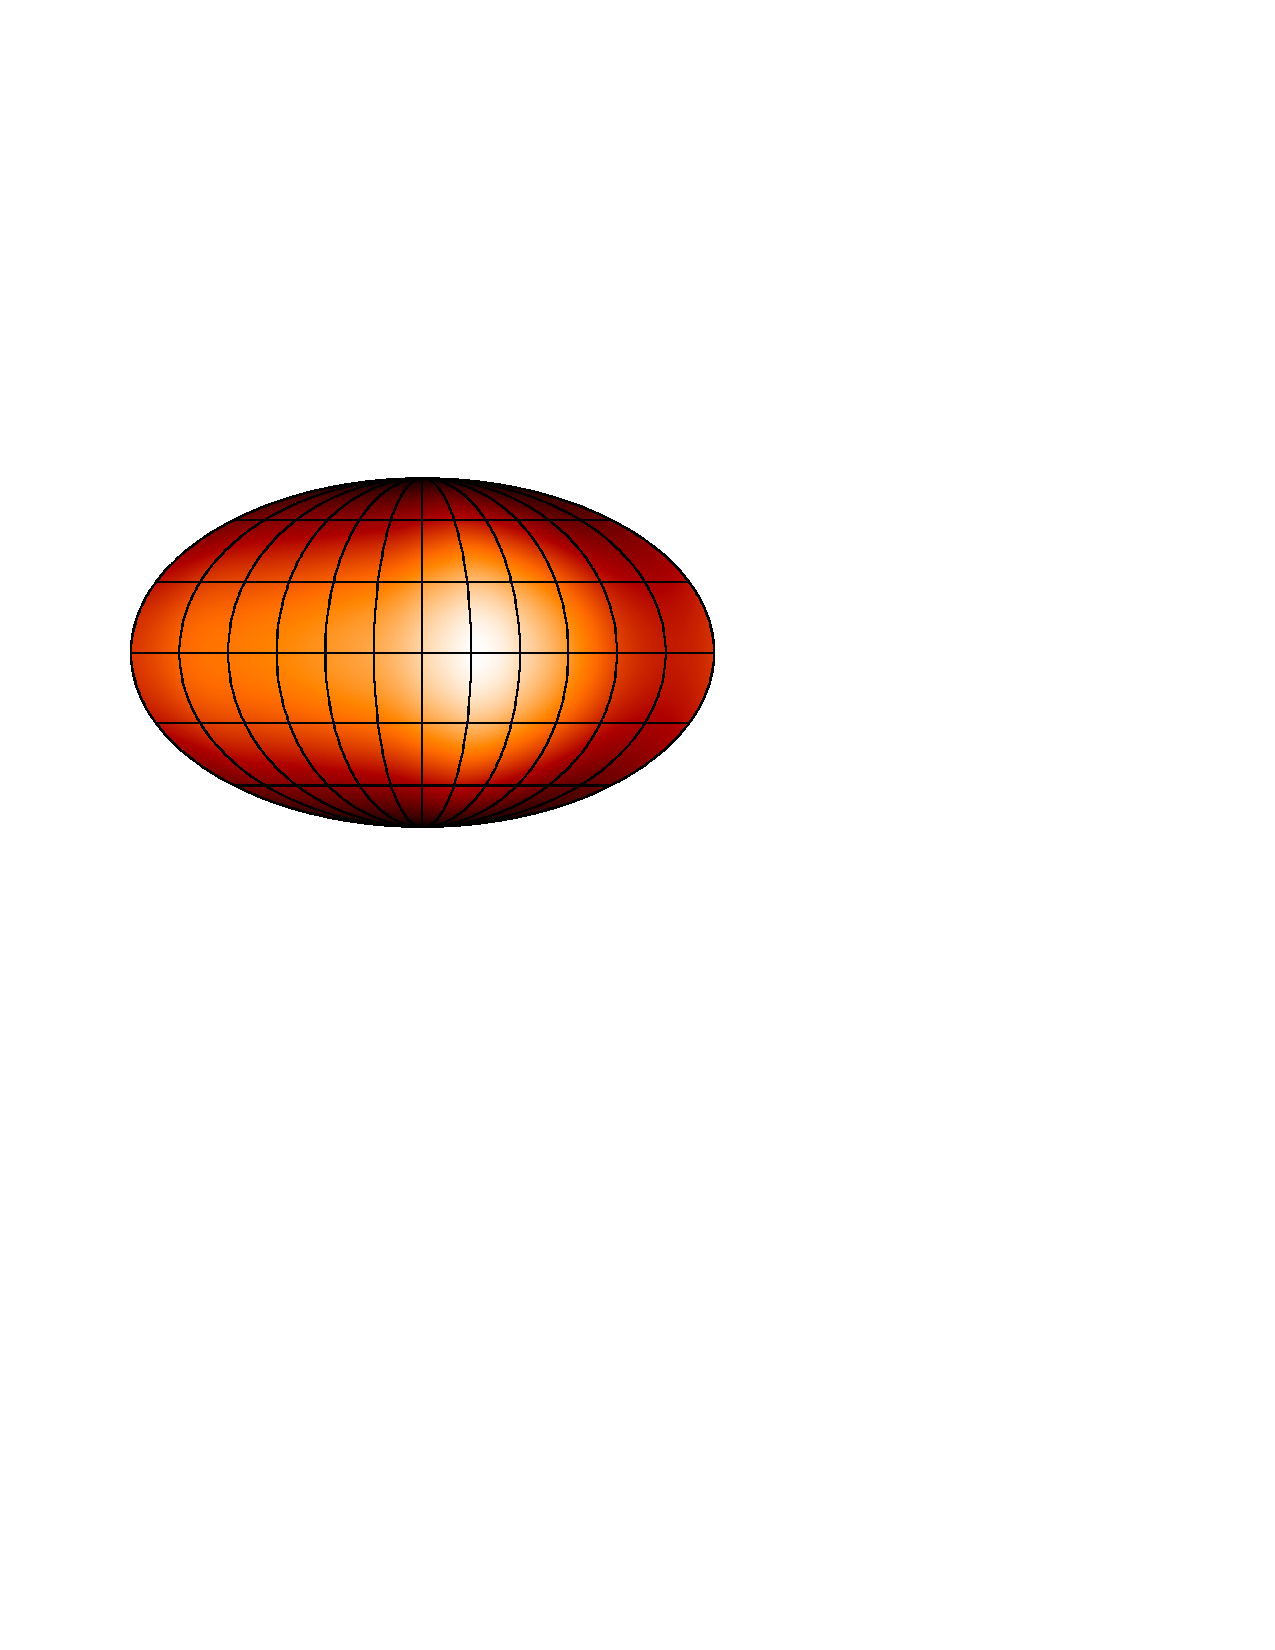
\includegraphics[width=0.4\linewidth]{figures/introduction/knutson_2007_temperature_map_HD_189733b.pdf}
    \caption[Exoplanet phase variations and temperature map.]{Left: Band integrated phase variation of {WASP-43b} from the HST~\citep{stevenson_thermal_2014}.
        The primary transit is inset top right.
        The peak of brightness occurs before the secondary transit.
        Right: Global temperature map of the hot Jupiter HD\,189733b obtained with {Spitzer Space Telescope}~\citep{knutson_map_2007}.
        The hottest point is offset from the sub-stellar point with the day side and night side temperatures around 930\K{} and 650\K{} respectively.}
    \label{fig:phasecurve2014_and_temp_map}
\end{figure}

Secondary transit and phase variations are an extension of the transit method, requiring higher precision to detect the reflection and thermal emission of the exoplanet.
The observed light curve is analysed considering it has two components, not only light from the star but also light from the planet, albeit at a much lower flux level.
To help visualize and discuss the components of exoplanet atmospheres \cref{fig:transits_and_occultations} is provided showing a transiting planet in orbit around a star, in which the planet also passes behind the star causing an occultation.
The planet is shown at several positions of the orbit indicating the proportion of day side and night side observed.
Below the star and planet is a diagram showing the changing flux variation (solid black line) over time, following the orbit.
If the orbital alignment is such that the planet will pass behind the star it will cause an occultation of the planet.
At this point the only light received is from the star alone, creating a baseline stellar measurement.
While during the primary transit there is also a small thermal emission contribution from the night side of the planet, as well as it partially blocking the star.

Throughout the orbit of the planet there is a variation in the planetary flux due to the alternating day/night side of the planet observed.
There are multiple components of the planetary flux, reflection and emission, that can be analysed with multi-band phase curves~\citep[e.g.][]{knutson_characterizing_2009, esteves_optical_2013}.
Optical phase curves will mostly show the reflected light from the day side of the planet, allowing modelling of the atmospheric albedo (fraction of light reflected by the atmosphere), and can provide details on the atmospheric scattering~\citep{madhusudhan_analytic_2012} and aerosol composition~\citep{oreshenko_optical_2016} through the optical phase function (day/night fraction).
Thermal emission of the planet will provide stronger modulation of infrared phase curves and can provide insights into the atmospheres thermal
structure and heat circulation~\citep{goodman_thermodynamics_2009, koll_temperature_2016}.

An example of phase variations in the infrared spectra of {WASP-43b} obtained with the Hubble Space telescope is given in \cref{fig:phasecurve2014_and_temp_map} (left).
The large amplitude of phase variation between the day and night side indicates that the night side is much cooler and there is an inefficient heat circularity from the day to night side.
A planet with an efficient day/night heat distribution mechanism would quickly equalize and have smaller phase variation.
One key observable from \cref{fig:phasecurve2014_and_temp_map} is that the peak of the phase variation is offset from the location of the secondary transit.
The hottest part of the atmosphere does not correspond to the sub-stellar point i.e.\ the point of the planet's surface closest to the star.
This is also observed in surface temperature mapping of the hot Jupiter HD\,189733b obtained with the {Spitzer Space Telescope}~\citep{knutson_map_2007} shown in the right of \cref{fig:phasecurve2014_and_temp_map}.
Simulations of atmospheric circulation models find that this offset is caused by super-rotating equatorial jets which move the location of the hottest point of the planet~\citep[e.g.][and references therein]{heng_atmospheric_2015}.

The point of occultation, at which the planet is completely blocked by the star, enables a baseline measurements for the star to be obtained without the planet.
\textbf{The depth of the occultation, is a direct measurement of the planet-to-star ratio between the star and the planet a }\todo{cite secondary eclipse of reflectance, and secondary spectroscopy examples}.
Spectra obtained during the occultation will have no planetary signal and can be used remove the stellar component from spectra obtained at other phases to obtain the planetary spectrum.


The depth of the occultation is a measure of the flux from the day side of the planet which can indicate the atmospheric reflection and thermal emission of the planet's atmosphere.


\subsection{Transmission spectroscopy}
\label{subsec:transmission_spectroscopy}
\begin{figure}
    \centering
    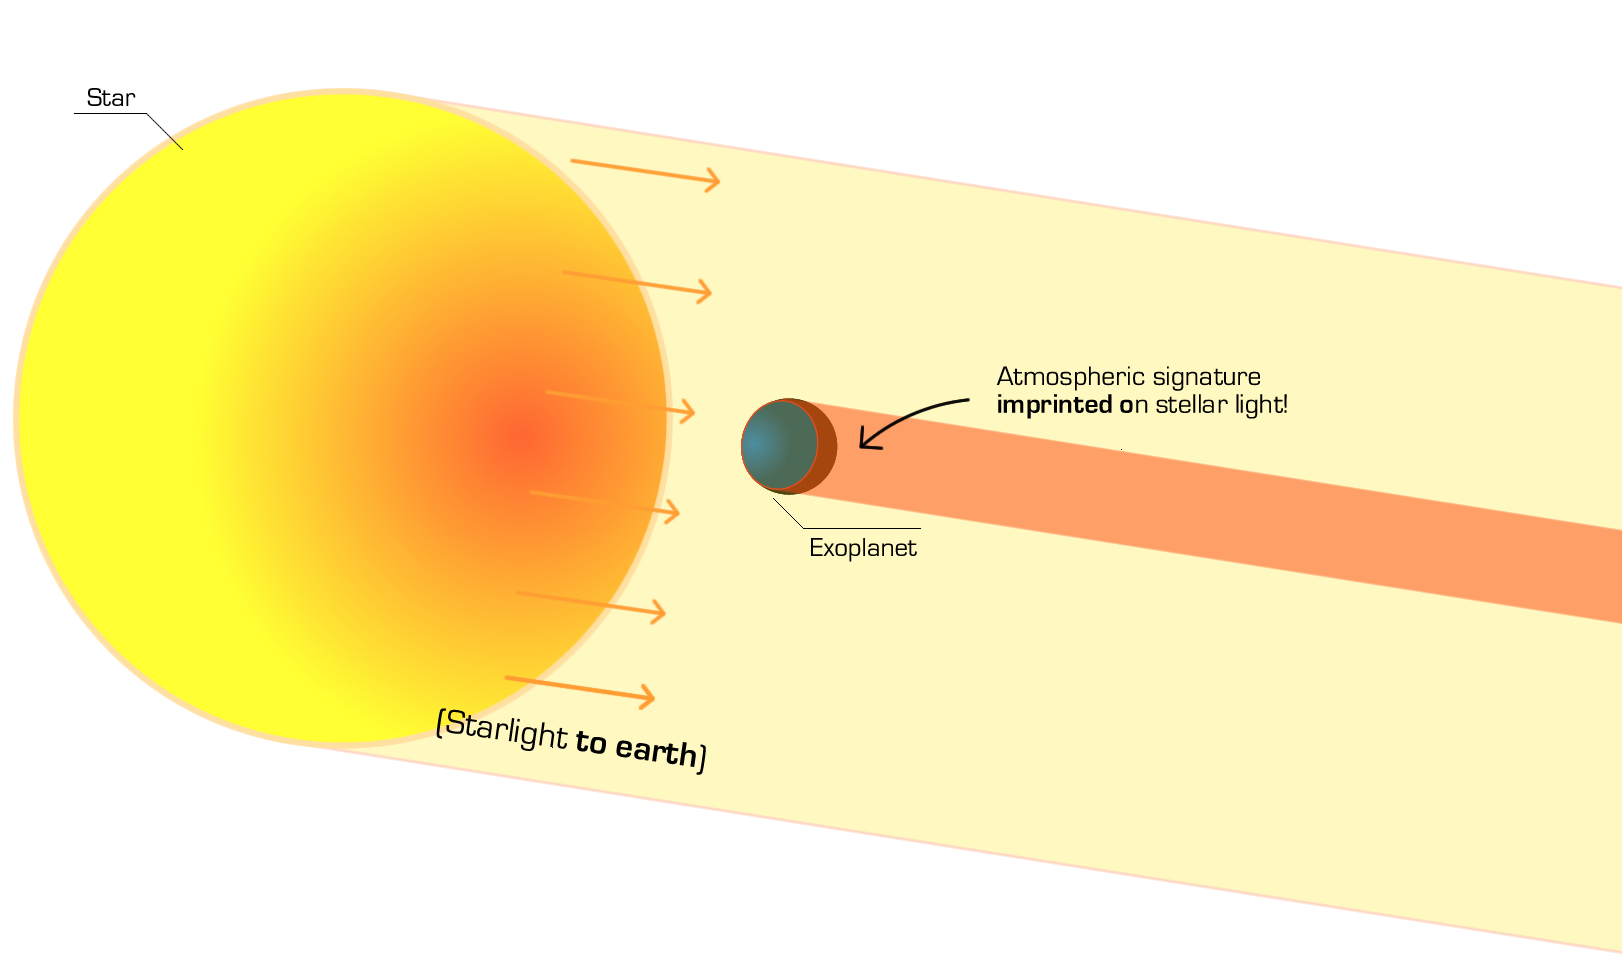
\includegraphics[width=0.65\linewidth]{figures/introduction/transmission_spectroscopy}
    \caption[Transmission spectroscopy diagram.]{Diagram of transmission spectroscopy imprinting the atmosphere of the exoplanet.
        Sourced from \href{http://www.sc.eso.org/~esedagha/research.html}{http://www.sc.eso.org/~esedagha/research.html}}
    \label{fig:transmissionspectroscopy}
\end{figure}

\begin{figure}
    \centering
    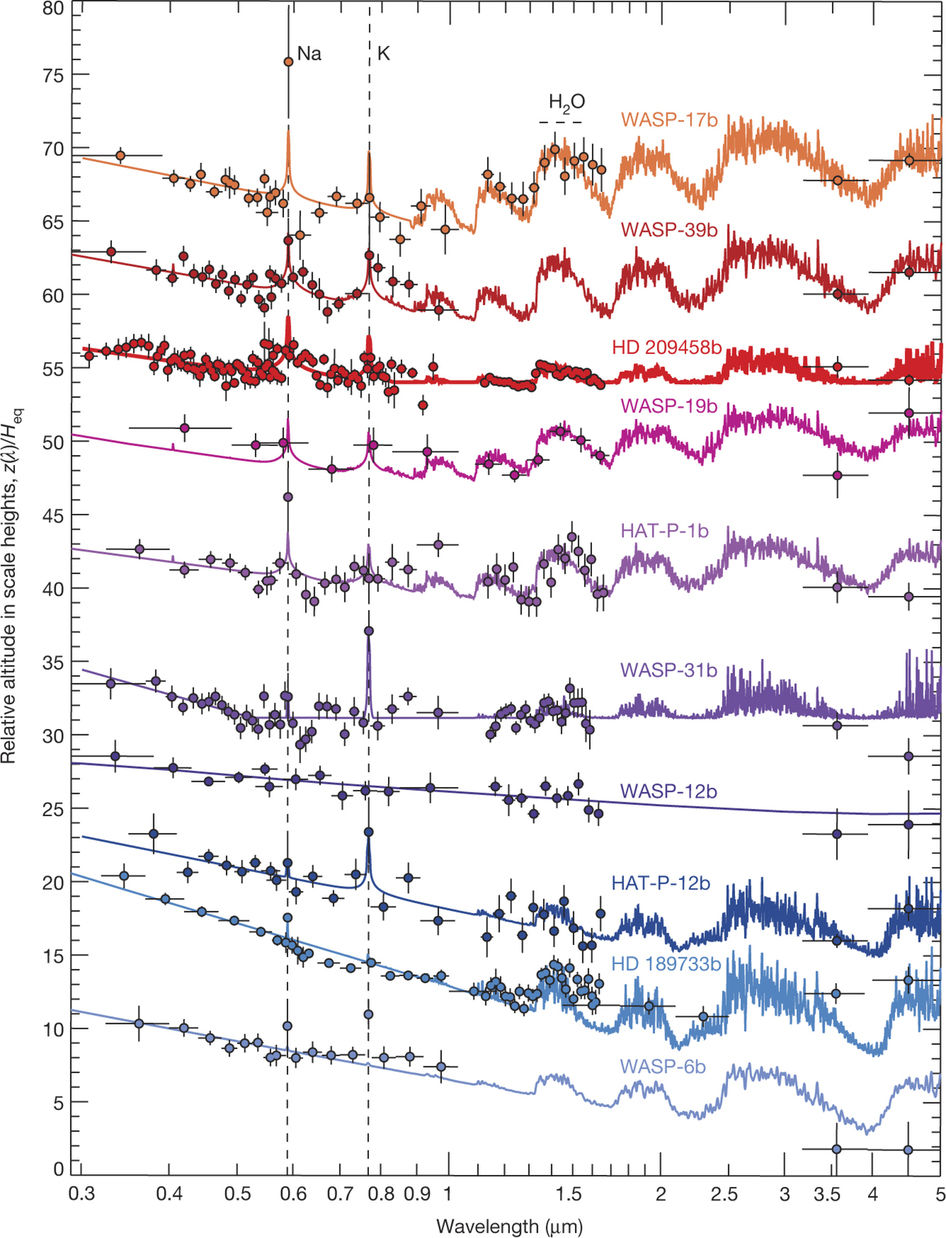
\includegraphics[width=0.6\linewidth]{figures/introduction/transmissionSpec_Sing2016}
    \caption[Transmission spectra for several Hot-Jupiter exoplanets.]{Transmission spectra (dots) for several Hot-Jupiter type exoplanets which increase in the amount of haze and clouds from top to bottom.
        The solid lines indicate the best fit atmospheric models.
        Credit~\citet{sing_continuum_2016}.}
    \label{fig:transmissionspecsing2016}
\end{figure}

When a transiting planet crosses in front of the host star it blocks out light from the star.
However, a small portion of light passes through the atmosphere of the planet as shown in \cref{fig:transmissionspectroscopy}.
The light that passes through the exoplanet atmosphere is partially absorbed, and is faintly imprinted with absorption lines.


In planetary transits, usually defined by their duration and depth, there are degeneracies in the transit shape from a single band, such as the \(\frac{\Rp}{\Rstar}\) ratio.
Observing transits in multiple bandpasses (i.e.\ by splitting the spectra observed during transits into several bands)  has been shown to break the degeneracies between the stellar radius and the orbital inclination as well as determine the stellar limb darkening~\citep{jha_multicolor_2000, knutson_using_2007}.

The radius of the transiting exoplanet can also appear to change size when observed at wavelengths where there is strong opacity in the atmosphere~\citep[e.g.][]{burrows_radii_2000, seager_theoretical_2000}.
Transits in different wavelength bands will have varying depths, dependant on the opacity of the atmosphere to each band. 

The transmission spectra observed with space observatories and ground based high resolution spectrographs have been able to detect several elements and molecules in the atmosphere.
For example \ce{Na}~\citep{charbonneau_detection_2002, redfield_sodium_2008, wyttenbach_spectrally_2015, nikolov_vlt_2016} \ce{H2O}~\citep{tinetti_water_2007, brogi_carbon_2014} \ce{CO}~\citep{brogi_carbon_2014, snellen_mass_2018}, \ce{CH4}~\citep{redfield_extrasolar_2010}, \ce{Fe} and \ce{Ti}~\citep{hoeijmakers_atomic_2018}.
The presence of clouds in the atmosphere have also been detected, as they mask the atmospheric constituents as they produce wavelength-independent fluxes~\citep[e.g.][]{barman_clouds_2011, kreidberg_clouds_2014, sing_continuum_2016}.

Transmission spectra for several transiting Hot-Jupiter exoplanets from~\citet{sing_continuum_2016} is shown in \cref{fig:transmissionspecsing2016}.
The amount of haze and clouds present in the atmospheres increases from top to bottom.
The clearer atmospheres near the top have large alkali lines (\ce{Na} and \ce{K}) and \ce{H2O}, while the cloudier planets lower down have strong optical scattering slopes, narrow alkali lines and partially or completely obscured \ce{H2O} absorption.


\subsection{High resolution spectroscopy}
\label{subsec:high_resolution_spectroscopy}

\begin{figure}
    \centering
    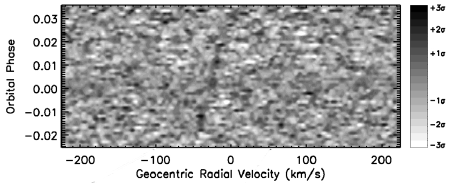
\includegraphics[width=0.7\linewidth]{figures/introduction/snellen2010}
    \caption[Cross-correlation signal from {CRIRES} observations of HD\,209458\,b.]{Cross-correlation signal of {CRIRES} observations during the transit of HD\,209458\,b with a \ce{CO} template.
        Credit~\citet{snellen_orbital_2010}.}
    \label{fig:snellen2010}
\end{figure}

Precise high resolution spectrographs, which are too large and bulky to fly in space, are able to spectrally resolve individual absorption lines, are key for analysing the atmospheres of exoplanets.
The large collecting area of current and future ground based telescopes make high resolution spectroscopy a great contender for obtained high-resolution observations for detecting and exploring exoplanetary atmospheres.

Typically high-resolution and high \snr{} are cross correlated with modelled planetary templates to recover the faint signal of the companion.
This has been most successful in the \nir{} due to the larger planet-to-star flux ratio
notably with CRIRES, with the detection of orbital motion, atmospheric constituents and exoplanetary winds~\citep[e.g.][]{snellen_orbital_2010, dekok_detection_2013, brogi_carbon_2014, brogi_rotation_2016, schwarz_evidence_2015}.
The rotation rate of exoplanets has been achieved by measuring the spectral line broadening~\citep{snellen_fast_2014, brogi_rotation_2016}.
An example of a cross correlated result is given in \cref{fig:snellen2010} showing the shift of the \ce{CO} lines during a transit due to the orbital motion of the planet~\citep{snellen_orbital_2010}.

The spectrum of the star and planet usually cannot be spatially resolved so methods to identify and remove the stellar component are required.
This usually involves constructing a high \snr{} stellar mask from observations, possibly at different phases~\citep[e.g.][]{rodler_weighing_2012}, to subtract from the observed spectra leaving behind the planetary signal.
If the planet is able to be spatially resolved, then a spectrum of the planet could be obtained without stellar contamination~\citep[e.g.][]{snellen_combining_2015}.

High resolution spectroscopy of atmospheres is not limited to transit spectroscopy with detections also possible for non-transiting exoplanets~\citep[e.g.][]{brogi_signature_2012, brogi_carbon_2014,lockwood_nearir_2014, piskorz_evidence_2016}.

An advantage of high-resolution spectra is that it allows the molecular absorption lines of Earth's atmosphere to be resolved.
This way they can be identified and corrected/removed to avoid contamination with the atmosphere of the exoplanet.
 Lower resolution and photometric methods are unable to fully resolve and remove Earth's atmosphere from ground based observations.



%!TEX root = ../../thesis.tex

\section{The diversity of exoplanets}

Exoplanetary detections have challenged the theoretical formation models with their variety and distribution of sizes and, locations.
For instance, the discovery of the hot-Jupiter class (large mass planets on close in orbits) challenged the accepted planet formation theories at the time~\citep[.e.g][]{pollack_formation_1996, boss_giant_1997} in which our Solar System was thought to be typical with small rocky planets close to the Sun and large giant planets further away.

The precise characterization of more exoplanets with the detection of exoplanetary atmospheres will allow for the constraints of exoplanetary composition and formation mechanisms to be improved.
For instance, the core accretion model has been able to reproduce the large number of Super-Earths, the correlation between star metallicity and planet frequency~\citep[e.g.][]{santos_spectroscopic_2004, fischer_planetmetallicity_2005}, and the presence of many Hot-Jupiter and Neptune like planets in close-in orbits, with the help of migration mechanisms~\citep[e.g.][]{triaud_exoplanets_2016}.
Recent models also combine both planetary formation and evolution to describe the observed exoplanets~\citep[e.g.][]{mordasini_characterization_2012} and can reproduce general population properties in a statistically significant way~\citep{mordasini_extrasolar_2009}.

A proxy for the composition and structure of an exoplanet is the average density, computed from the mass and radius.
A mass-radius diagram is shown in \cref{fig:santerne2018} for Earth-like rocky planets.
The tracks show contours of mass-radius for different theoretical compositions~\citep{brugger_constraints_2017}, while the circles indicate a number of detected small mass exoplanets, with {K2-229\,b} being a Super-Earth with a Mercury-like density~\citep{santerne_earthsized_2018}.
The density can give an approximate composition but for a given mass there are an infinite number of combinations of metal/silicate/ice and gas that can produce the same radii~\citep[e.g.][]{seager_massradius_2007}.
Low mass planets tend to be rocky and tend to have small or no atmosphere.
With rock being in-compressible, to first order, it is relatively insensitive to the incident flux.
The radii of solid exoplanets are sensitive to gas content of the atmosphere as a small increase in \ce{H} and/or \ce{He} can cause a large increase in radius~\citep{adams_ocean_2008}.

\begin{figure}
    \centering
    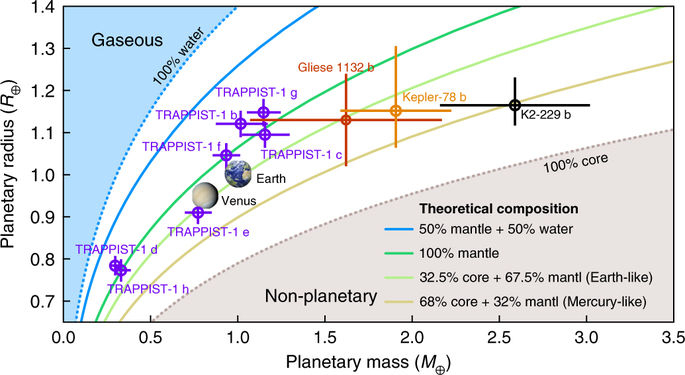
\includegraphics[width=0.7\linewidth]{figures/introduction/santerne_2018}
    \caption[Mass-Radius diagram for rocky planets with composition contours.]{Mass-Radius diagram for rocky planets with composition contours.
        Adapted from~\citet{santerne_earthsized_2018}}
    \label{fig:santerne2018}
\end{figure}

When the gas component becomes dominate, planets begin to have radii independent of their mass~\citep[e.g.][]{lopez_understanding_2014}.
The atmospheres of gas giants are also susceptible to stellar irradiation, with close in Hot-Jupiters having inflated atmospheres and larger radii~\citep[e.g][]{fortney_interior_2010}.


\begin{figure}
    \centering
    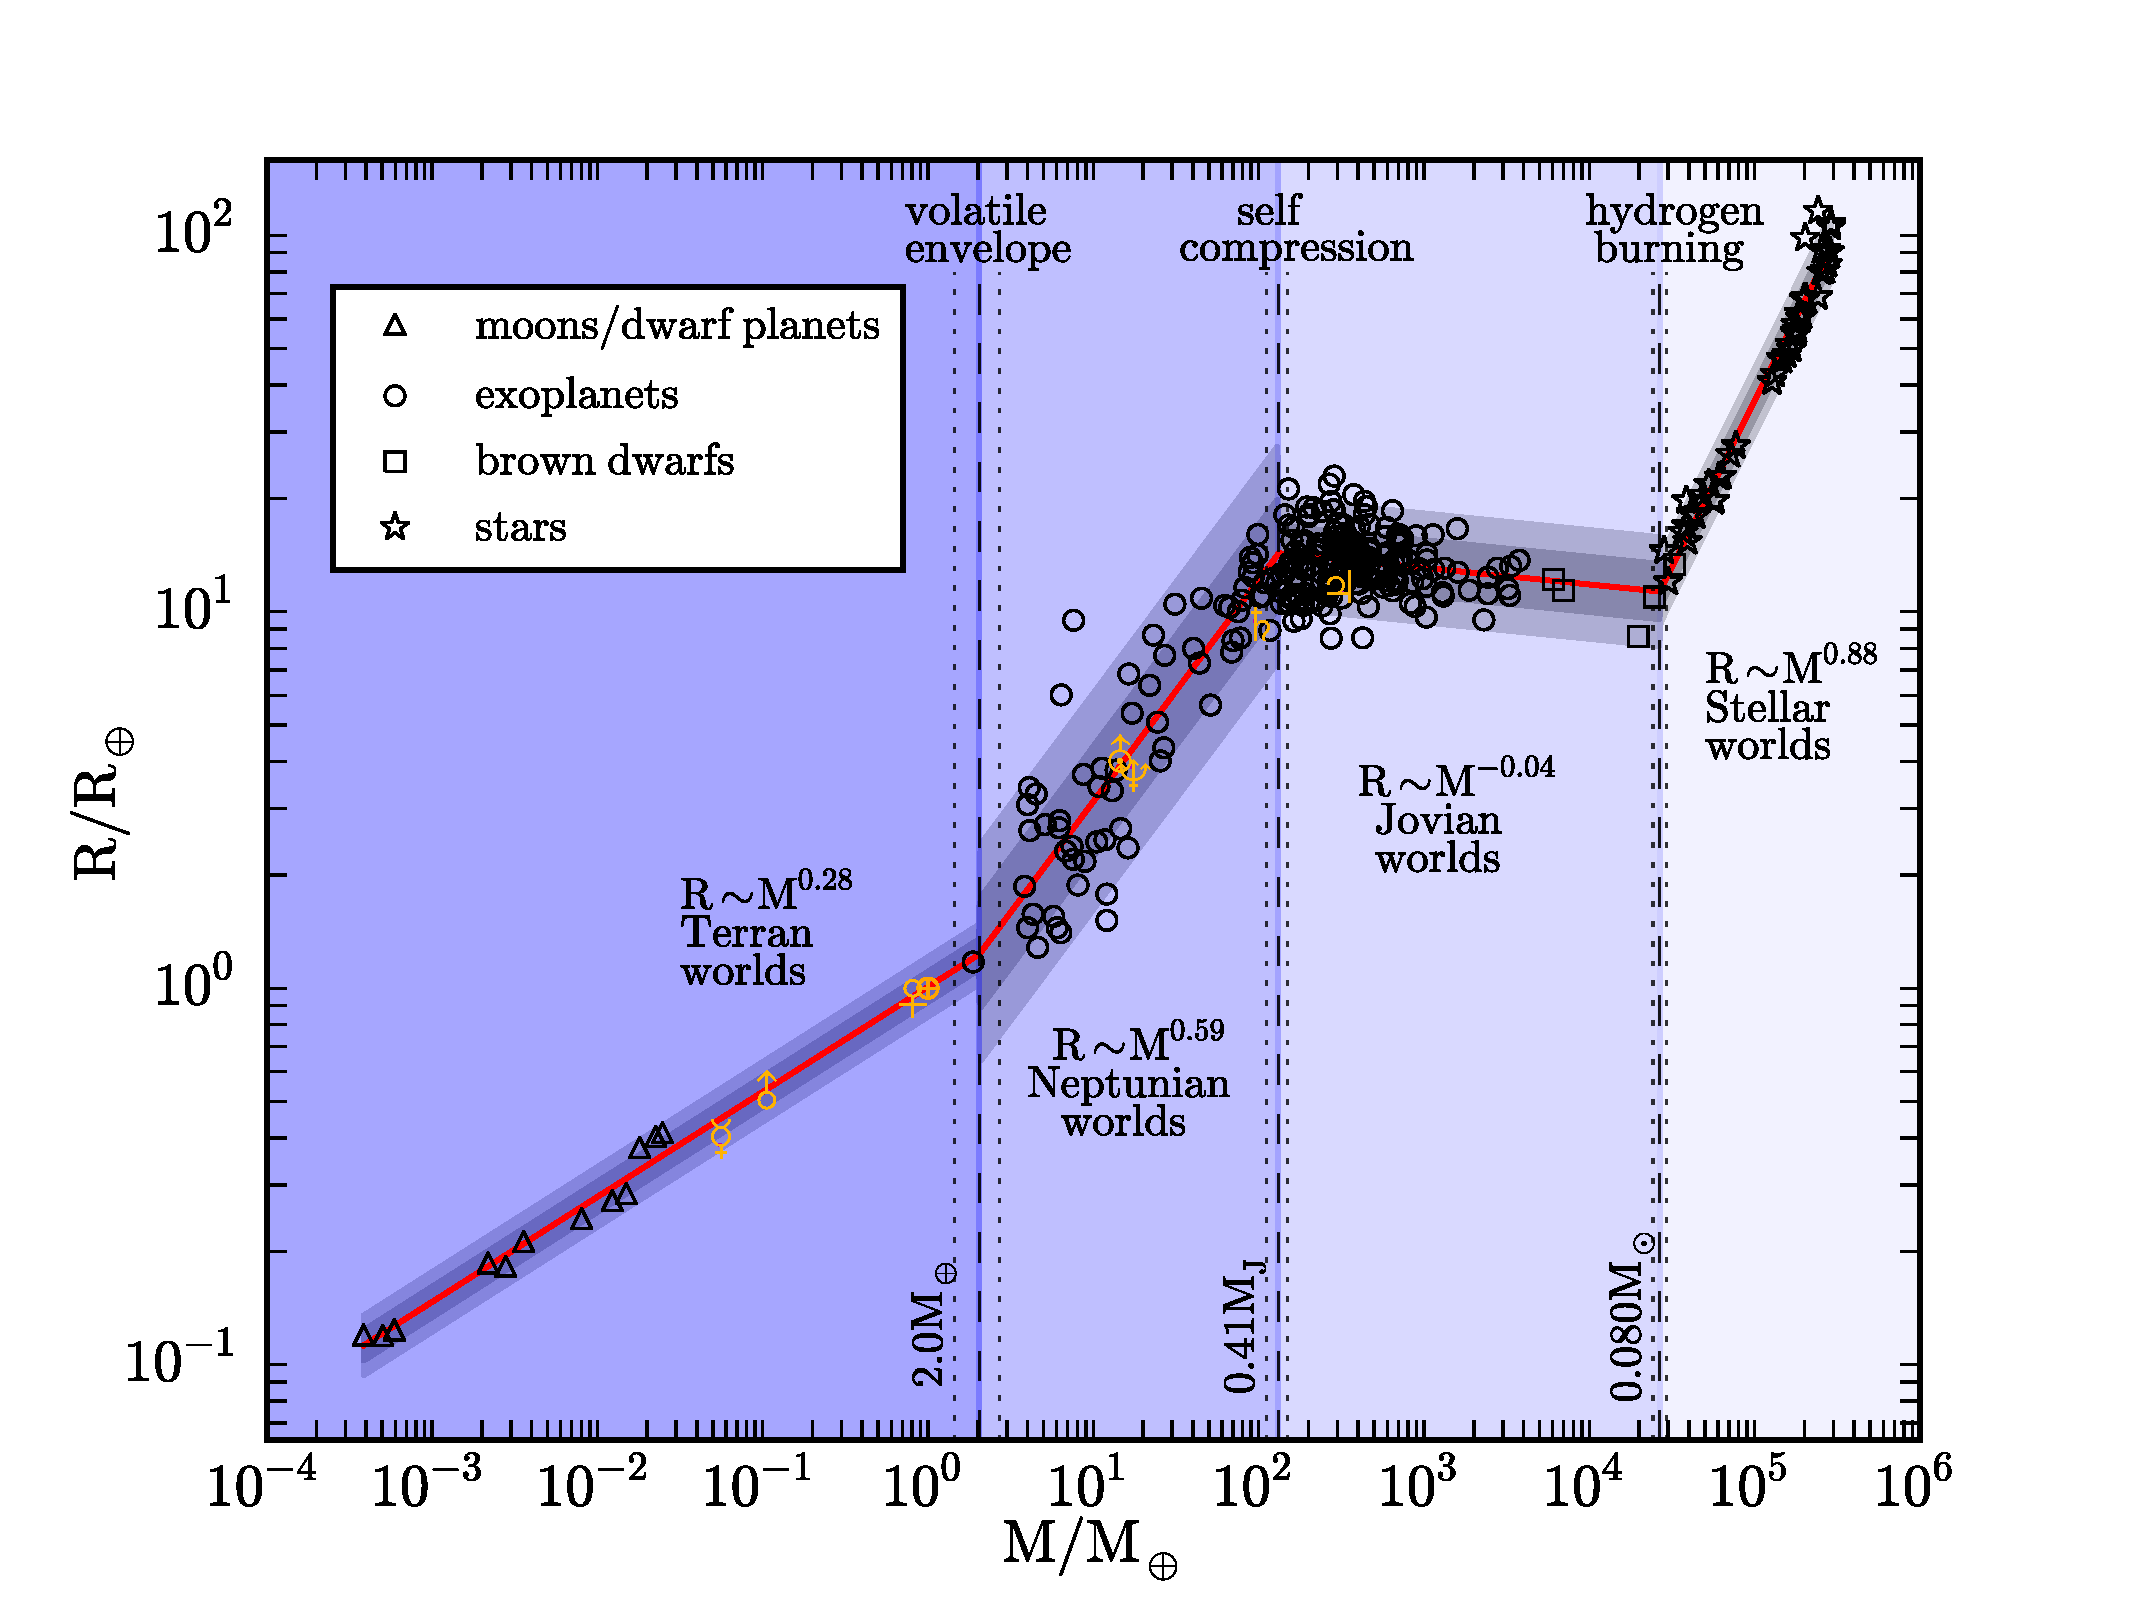
\includegraphics[width=0.7\linewidth]{./figures/introduction/mass_radius_relation.pdf}  \\
    \caption[Mass-Radius relationship with probabilistic fit.]{Mass-Radius relationship with probabilistic fit from dwarf planets to late-type stars from~\citet{chen_probabilistic_2016}.
    The black symbols represents the objects used to fit the model, with the key in the top-left, while the orange symbols represent the solar system planets.
    The red line indicates the average value, while the light and dark grey regions indicate the 65\% and 95\% confidence intervals.}
    \label{fig:mass_radius_relation}
\end{figure}

Models of the mass-radius relation are important as they enable insight into the likely planetary properties when only either mass or radius can or has been measured.
For example~\citet{chen_probabilistic_2016} developed a probabilistic model over 9 orders-of-magnitude in mass and 3 orders-of-magnitude in radius, with the result shown in \cref{fig:mass_radius_relation}.
There are four separate power laws and three different transition regions fitted by the model.
This breaks the mass radius relation into different regions classified after a representative example from our solar system.
The lowest mass range is the rocky "Terran" worlds up to 2.0\,\(\textrm{M}_oplus\) and inclusive of dwarf planets, "Neptunian" worlds between 2.0,\(\textrm{M}_oplus\) and 0.41\,\Mjup{} and, "Jovain" worlds between 0.41\,\Mjup{} and 0.08\Msun{}.
The transitions regions are indicative of a changing composition or physical processes (such as the hydrogen burning limit in stars) and consistent with other works~\citep[e.g.][]{weiss_mass_2013, dieterich_solar_2014, hatzes_definition_2015, rogers_most_2015}.

Recently, there has been a renewed interest in Brown Dwarf (BD) candidates triggered by exoplanetary searches as they bridge the gap between giant planets and low-mass stars.
It is difficult to distinguish between giant planets and BDs with a loosely suggested definition of mass between 13--80\,\Mjup{}\footnote{0.01--0.08\Msun{}} for Brown Dwarfs as this is between the Deuterium fusion mass of around 13\,\Mjup{}~\citep[e.g.][]{spiegel_deuteriumburning_2011} and the Hydrogen fusion limit of 80\,\Mjup{}~\citep{chabrier_theory_2000, dieterich_solar_2014}.
Several works found similar properties on the two populations, like a similar density~\citep{hatzes_definition_2015, chen_probabilistic_2016} seen in \cref{fig:mass_radius_relation} by the same power law spanning giant planets and BDs, while others have found intriguing differences.
When classified using just mass and size~\citet{chen_probabilistic_2016} find no difference between giant planets and Brown Dwarfs, with Brown Dwarfs just being large giant planets.

There is a paucity of {BD} companions in short period orbits around Sun-like stars (\(\lesssim{}5 \)\AU{}), compared to stellar or planetary companions, termed the \emph{brown dwarf desert}~\citep{halbwachs_exploring_2000, zucker_analysis_2001, sahlmann_search_2011, ranc_moa2007blg197_2015} which can been seen as the gap in the "Jovian" worlds section of \cref{fig:mass_radius_relation}.
There are observed differences in the host star metallicity~\citep{maldonado_searching_2017, santos_observational_2017, schlaufman_evidence_2018} and orbital eccentricity distribution~\citep{ma_statistical_2014} either side of the period/mass gap with the lower mass BDs having properties similar to giant planets and high mass BDs having properties more like stars.
There is a very strong hint of different formation mechanisms as BDs below the gap may primarily form via gravitational instability in protoplanetary disks, while above this gap BDs may form more like stellar binary from molecular cloud fragmentation~\citep{ma_statistical_2014}.

As the number of known BDs orbiting solar type stars is low, the characterization of benchmark BDs in the brown dwarf desert~\citep[e.g.][]{crepp_trends_2016} is beneficial in understanding this sub-stellar population and to help constrain formation and evolution theories~\citep{whitworth_formation_2007}.
There is an inherent degeneracy between the mass, age and luminosity of a given BD~\citep{burrows_nongray_1997} because without sustained fusion, BDs cool down over time with an age-dependent cooling rate.

BDs in binary systems, unlike free-floating BDs~\citep[e.g][]{gagne_simp_2017}, allow for the determination of their masses, when complemented with radial velocity ({RV}) and astrometry measurements.
The {RV} technique provides the mass lower-limit (\Mtwosini{}) of binary and planetary companions, while complementary astrometry measurements can often provide mass upper-limits~\citep[e.g.][]{sahlmann_search_2011}.
Measuring or tightening the constraints of {BD} masses improves the understanding of mass dependence on {BD} formation processes.
Photometry along with stellar evolution models~\citep[e.g.][]{baraffe_evolutionary_2003,allard_btsettl_2013} can also be used to estimate the mass of {BD} companions~\citep[e.g.][]{moutou_eccentricity_2017} if there is sufficient orbital separation, and a precise determination of the age~\citep{soderblom_ages_2010}.


%
%\begin{figure}[t]
%    \centering
%    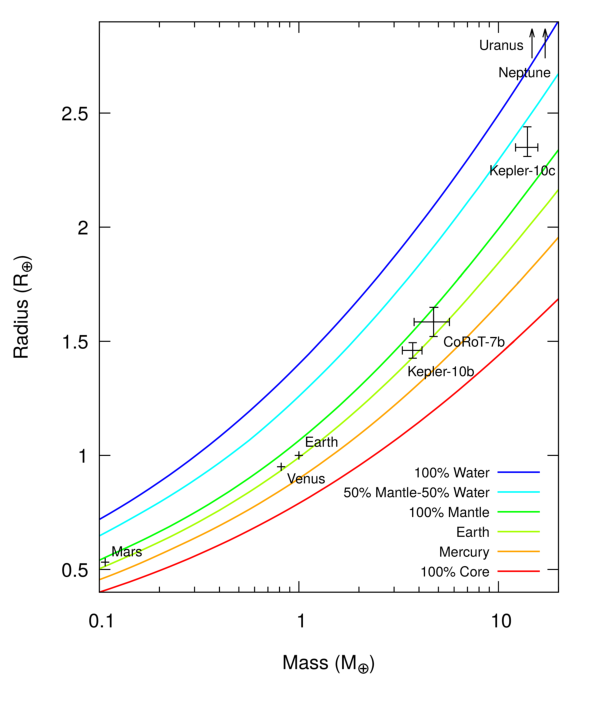
\includegraphics[width=0.4\linewidth]{./figures/introduction/Mass_radius_relation-compostion_Brugger_2017.pdf}
%    \caption[]{Mass-Radius relationship for (super) Earth-like planets with composition contours.
%        Adapted from~\citet{brugger_constraints_2017}}
%    \label{fig:mass_radius_relation_composition}
%\end{figure}
%
%
%
%\begin{figure}
%    \centering
%    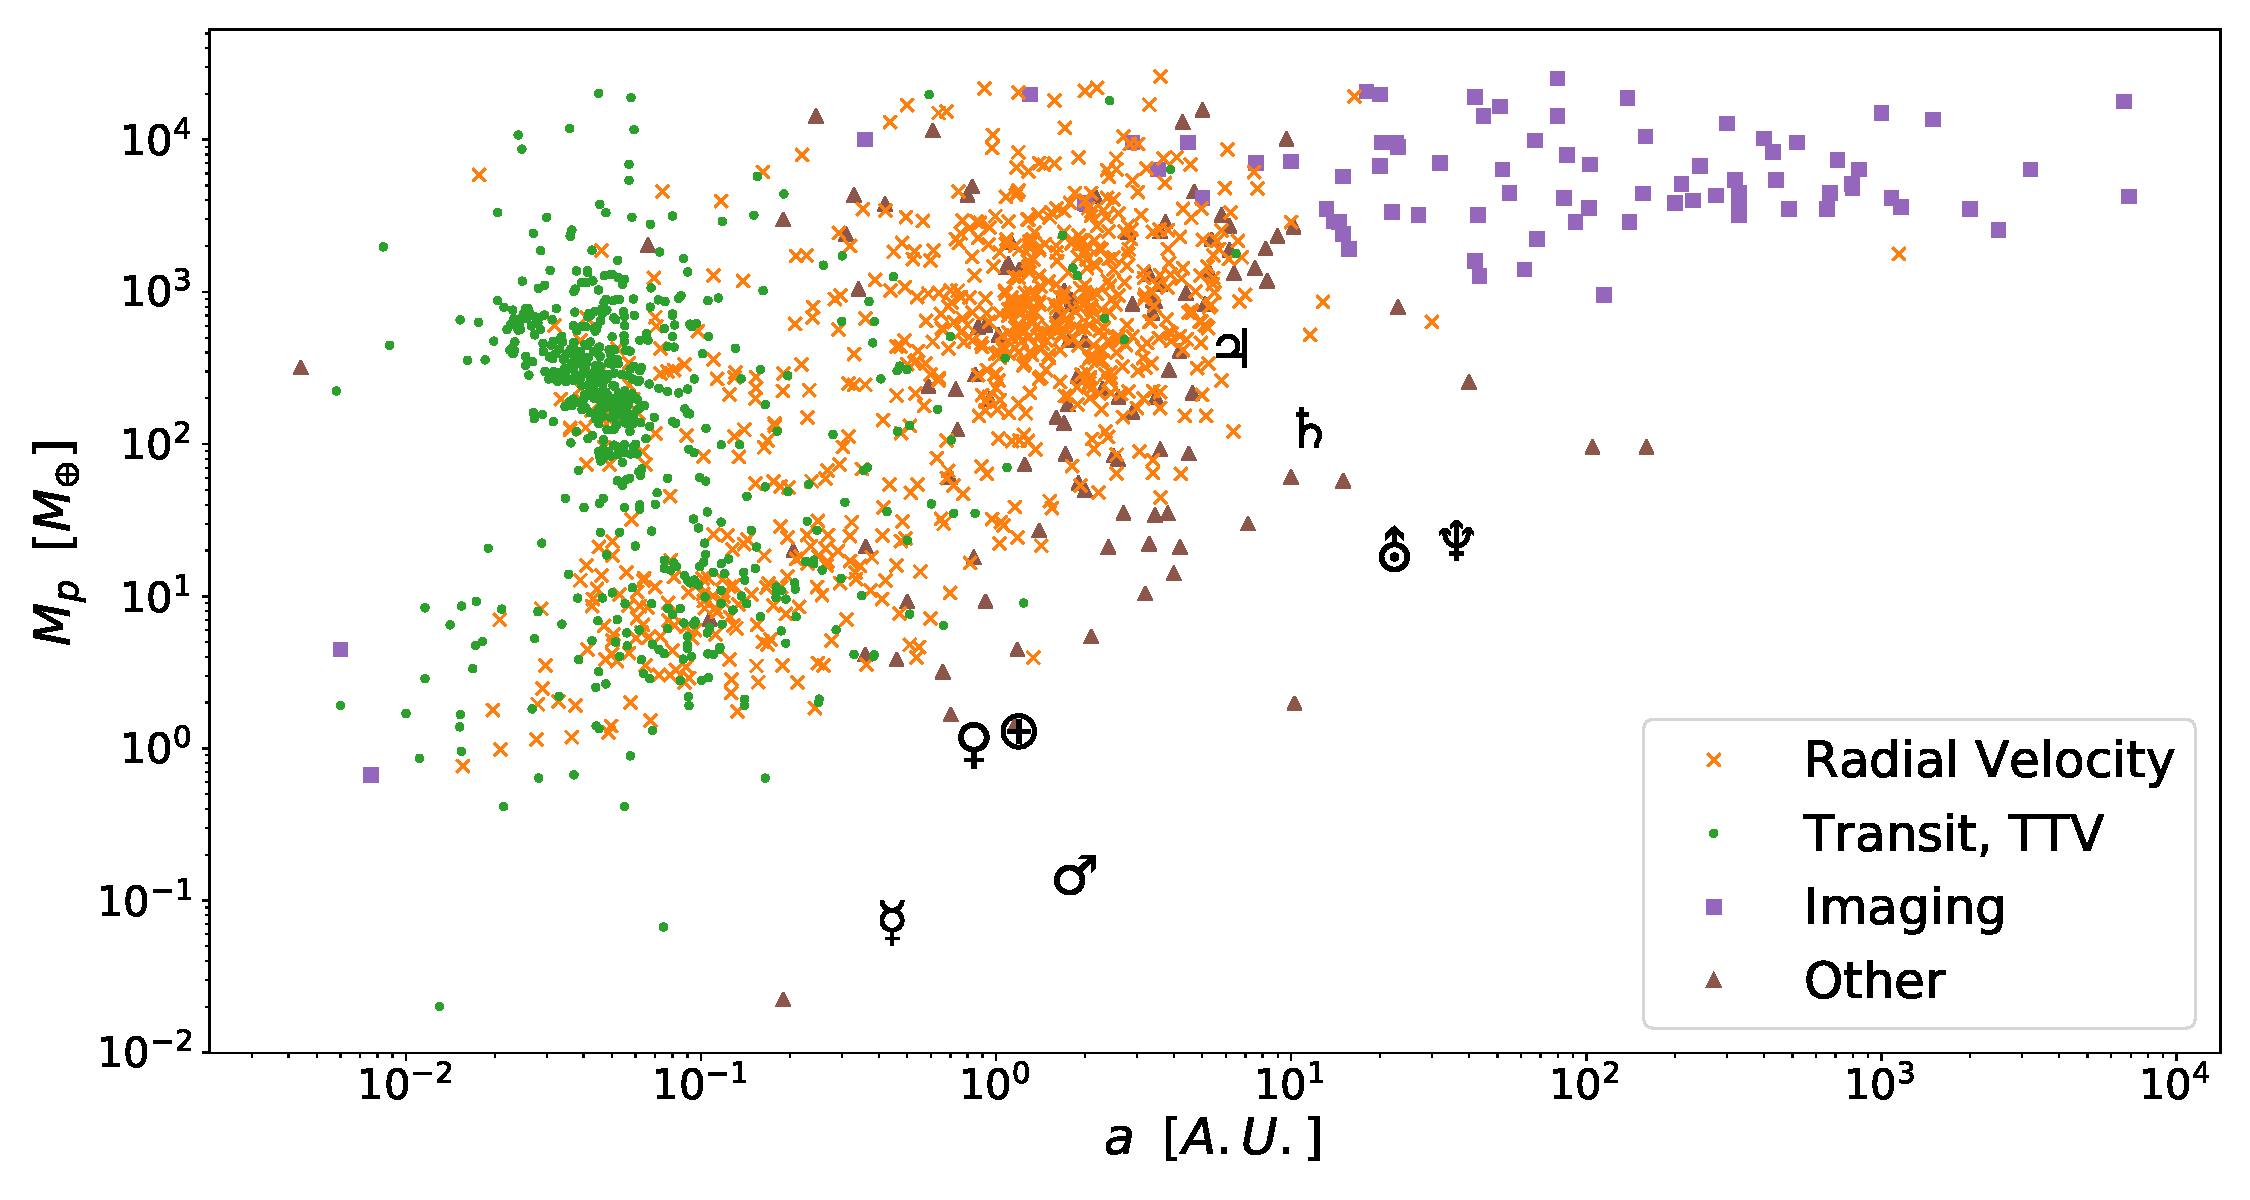
\includegraphics[width=0.\linewidth]{./figures/introduction/exoplanetEU_a_mass.pdf}
%    \caption[]{Exoplanet semi-major axis verses mass diagram.
%        The symbols indicate the location of the solar system planets, $\mercury$-Mercury, $\venus$-Venus, $\earth$-Earth, $\mars$-Mars, $\jupiter$-Jupiter, $\saturn$-Saturn, $\uranus$-Uranus, $\neptune$-Neptune.
%        Data from \href{http://ww.exoplanet.eu}{exoplanet.eu} October 2018}
%    \label{fig:pltoverlayadd}
%\end{figure}
%
%
%Explore what these method have found with exoplanet populations.





\subsection{Model fitting transit stars (not actual title, more other similar methods)}
There are other situations in which to determine the presence of faint secondary spectra, such as identifying the presence of any background or companion stars of transiting planet candidates.
Many astronomical phenomena such as grazing eclipsing, a giant primary star eclipsed by a dwarf or a background star can produce signals indistinguishable from planetary transits.
Efforts to characterize the false positive probability (FPP) among Kepler planet candidates is as high as $\sim35\%$~\citep{santerne_sophie_2012}.
The presence of unknown companions or background stars decreases the dimming effect from the planet transit leading to smaller planetary radius.
Where multiple stars are present there may also be ambiguity on which star hosts the planet.
\citet{kolbl_detection_2015} developed a method for detecting the presences of faint secondary lines in optical stellar spectra by matching observations to the SpecMatch library of stellar spectra.
Identifying the spectroscopic evidence of a secondary star for 63/1\,160 California \emph{Kepler} Survey objects of Interest (KOI).


For transiting planets, the presence of a background star or a companion star causes problems in characterizing the planet.
Being able to detect spectra signal of the a faint second spectra in double-lined spectroscopic binaries.
For example eclipsing binaries,
A dim binary system companion or a giant planet around a background star can mimic the transit of a small Earth-like planet on a foreground star.






\subsection{Earth's atmosphere}
\todo{move out of intro}
While the Earth's atmosphere is important for an Astronomer's lungs, it can be a nuisance for their ground-based observations.
As light form astronomical sources passes through the atmosphere, its molecular components absorb some of the light, changing spectral components observed by imprinting a transmission spectrum of our atmosphere.
The \ce{H2O} absorption is a key example as it defines the photometric and spectroscopic bands in the \nir{}. \missingfigure{example to point to}.

The correction of observations from the contamination of Earth's atmosphere is a complex process.\textbf{
The transmission is variable on many different time scales, the water vapour change is rapid, concentrations of atmospheric constituents, to seasonal and longer.}
Such as the increase in atmospheric \ce{CO2} causing anthropamorphic climate change this requires 6\% change to \ce{CO2} line depths since 2000 Molecfit paper?
There is also variation with airmass, which depends on the observation angle in the sky and changes as targets move across the sky during the night.

other constituents, \ce{CO}, \ce{CO2}, \ce{CH4} \ldots{}, angle of observations.

An important consideration in detecting the constituents of planetary atmospheres is the characterization and removal of Earth's telluric lines.

e.g.\ 50\% error in \ce{CO2} detection on Mars atmosphere


Recently~\citet{ulmer-moll_telluric_2018} compared the telluric correction possible from three different synthetic telluric software against the standard star model.
Molecfit, a software from ESO was the most.

This is a growing field and there are other software available too\ldots{}


Water vapour content has rapid variability.
Works such as Snellen 2011, \ldots{} \ldots{} model the telluric variation during a observations to remove telluric lines and detect planetary lines.

\todo{finish this}


Telluric absorption map
\begin{figure}
    \centering
    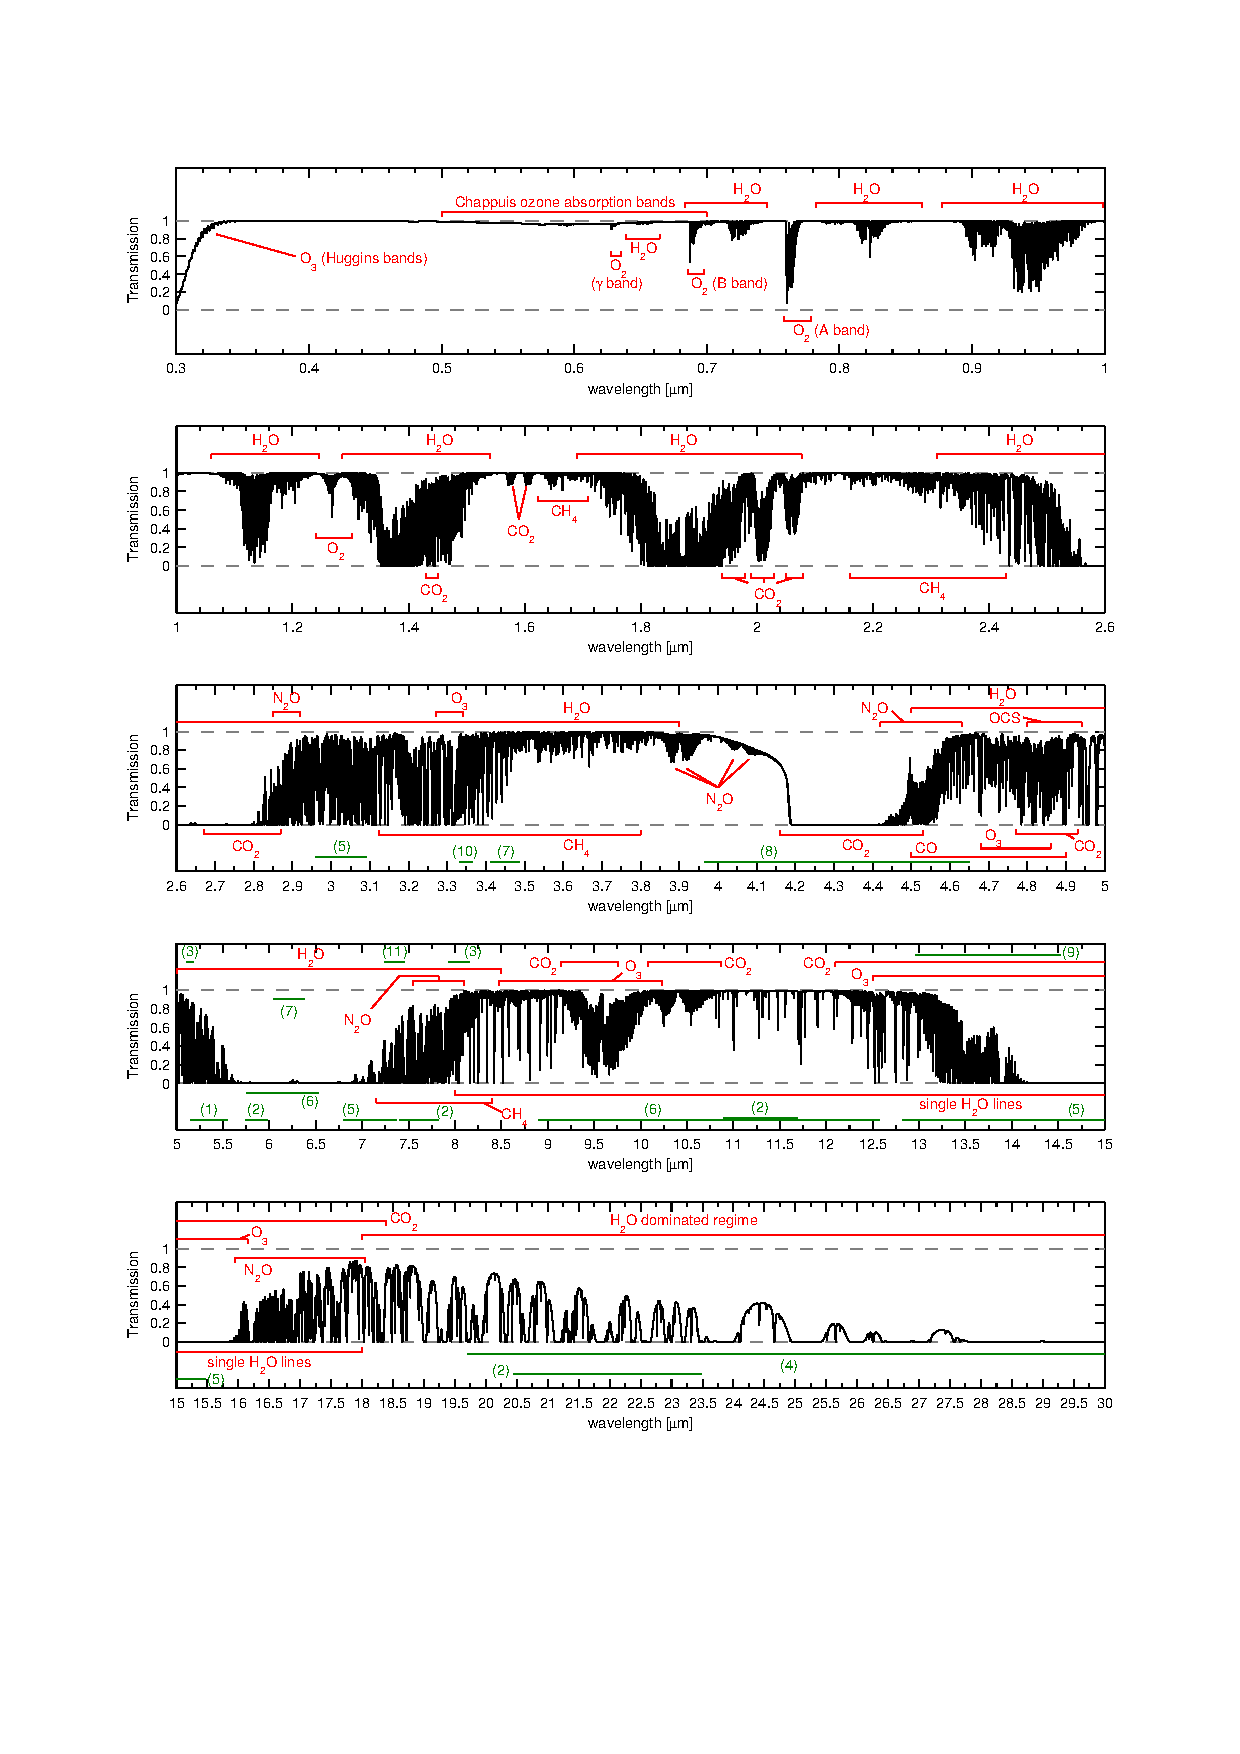
\includegraphics[width=0.9\linewidth]{figures/advanced_material/cropped_molecfit_absorbtion}
    \caption{Reproduction of Figure~1 of~\citet{smette_molecfit_2015} showing telluric absorption form 0.30 \um. Original caption:}
    \label{fig:croppedmolecfitabsorbtion}
\end{figure}
\todo{Add original caption to~\ref{fig:croppedmolecfitabsorbtion}}




\section{Paper Introduction}\label{sec:intro}
Brown dwarfs (BDs) are sub-stellar objects unable to achieve hydrogen fusion, with masses around \(13-80~\textrm{M}_{jup} \)~\citep{chabrier_theory_2000}, bridging the gap between low-mass stars and giant planets.
Without sustained fusion, brown-dwarfs cool down over time with an age-dependent cooling rate.
Therefore, there is an inherent degeneracy between the mass, age and luminosity of a given BD~\citep{burrows_nongray_1997}.
This degeneracy may be resolved by the observation of several parameters, for instance when a BD is in a binary system with a main sequence host star, using both the host stars age and the masses derived from the dynamical motion.

A paucity of BD companions exists in short period orbits around Sun-like stars (\(\lesssim5 \)\AU), compared to stellar or planetary companions, termed the \emph{brown dwarf desert}~\citep{halbwachs_exploring_2000, zucker_analysis_2001, sahlmann_search_2011}.
As the number of known BDs orbiting solar type stars is low, the characterization of benchmark BDs in the brown dwarf desert~\citep[e.g.][]{crepp_trends_2016} is beneficial in understanding this sub-stellar population and to help constrain formation and evolution theories~\citep{whitworth_formation_2007}.
The BD desert also provides a greater challenge as it reduces the amount of good BD candidates to study.

BDs in binary systems, unlike free-floating BDs, allow for the determination of their masses, when complemented with radial velocity ({RV}) and astrometry measurements.
The {RV} technique provides the mass lower-limit (\mtwosini{}) of binary and planetary companions, while complementary astrometry measurements can often provide mass upper-limits~\citep[e.g.][]{sahlmann_search_2011}.
Measuring or tightening the constraints of BD masses improves the understanding of mass dependence on BD formation processes.
For instance, there is growing evidence that the larger giant planets and BD companions do not follow the well known metallicity-giant planet correlation seen in main-sequence stars with planets~\citep[e.g.][]{santos_spectroscopic_2004,santos_observational_2017, maldonado_searching_2017}.
Photometry along with stellar evolution models~\citep[e.g.][]{baraffe_evolutionary_2003,allard_btsettl_2013} can also be used to estimate the mass of BD companions~\citep[e.g.][]{moutou_eccentricity_2017} if there is sufficient orbital separation, and a precise determination of the age~\citep{soderblom_ages_2010}.

Recently, there has been a renewed interest in BD candidates triggered by exoplanetary searches.
While several works found similar properties on the two populations, like a similar density~\citep{hatzes_definition_2015}, others found intriguing differences.
One of the most recent is the different host metallicity of the Brown Dwarf and giant planet populations~\citep{santos_observational_2017, schlaufman_evidence_2018}, a very strong hint of different formation mechanisms.

Spectral observations of binary systems contain the spectra of both bodies, in proportion to their flux ratio, and Doppler shifted relative to each other due to their orbital motion.
One technique to recover the spectra of the companion is secondary reconstruction through a differential spectrum~\citep{ferluga_separating_1997}.
Spectra from different phases are shifted to the rest frame of the host star and subtracted to mutually cancel out the spectrum of the host star allowing the faint companion spectra to become visible.
Advances in high-resolution and near-infrared (\nir{}) capabilities should enable this technique to be applied to BDs and planet companions, in which smaller {RV} shifts can be resolved and the contrast ratio of the smaller companion is improved.

Observing in the \nir{} is specifically desirable for the cooler sub-stellar and giant planet companions as their thermal emission is stronger in the infrared compared to the optical. This improves the contrast ratio between the host star and companion, providing favourable conditions for their detection and spectral separation.
CRIRES, a high resolution \nir{} spectrograph, has made many prominent advances in recent years with the detection of atmospheric constituents, such as \(\textrm{CO} \) and \(\textrm{H}_{2}\textrm{O} \), atmospheric winds and thermal profiles, rotation and orbital motion, for both transiting and non-transiting planets~\citep[e.g.][]{snellen_orbital_2010, brogi_signature_2012, rodler_weighing_2012, dekok_detection_2013, brogi_carbon_2014, snellen_fast_2014, piskorz_evidence_2016, brogi_rotation_2016, birkby_discovery_2017}.

The higher temperature and relatively larger size of BDs compared to giant-planets makes the development of spectral recovery techniques for BD companions a logical step towards the spectroscopic detection of planetary atmospheres.
There has been the recent installation and continued development of many new high-resolution \nir{} spectrographs, such as {CARMENES}~\citep{quirrenbach_carmenes_2014}, NIRPS~\citep{bouchy_nearinfrared_2017} or SPIRou~\citep{artigau_spirou_2014}, as well as, the {CRIRES+}~\citep{dorn_crires_2016} upgrade.
These new instruments motivate the study of \nir{}-oriented methodologies for spectral recovery, and are of high importance due to the larger planet-to-star flux ratio provided by near-IR compared to the visible.

{\rd{} The search and detection of faint secondary spectra is not only relevant to planetary atmospheres.
\citet{kolbl_detection_2015} developed a method to detect the presence of optical secondary spectra down to a flux ratio of 1\% in the hosts of \emph{Kepler} transit candidates.
The presence of which can cause ambiguities in the system configuration, and increase the uncertainty of the measured planet radius.
The characterization of the false positive probability rate for Kepler has been found to be as high as \(\sim\)35\%~\citet{santerne_sophie_2012}.}

In this paper we apply two different techniques on FGK stars with BD companions with the aim to spectroscopically detect their companions.
In \sref{sec:data} we present the observations and reduction process as well as the spectral models used in this work.
In \sref{sec:specdiff} we explain the differential spectral technique and its applicability to these observations while in \sref{sec:results} we apply companion recovery using a \textchisquared{} approach.
In \sref{sec:discussion} we discuss our results and in \sref{sec:conclusions} we present our conclusions.



brown dwarf dessert explore \citet{ranc_moa2007blg197_2015}

%!TEX root = ../../thesis.tex
\clearpage
% Motivation of this work
\section{Motivation}
\label{sec:motivation}

As shown in this introduction there is a vast field of exoplanet research, with one of the current challenges being the detection of planetary atmospheres, in the near infrared specifically. The purpose of this thesis is to develop methodologies and tools to extract he minute signals of planetary spectra from \nir{} spectra. Having access to \nir{} CRIRES spectra of stars with suspected Brown Dwarf companions\footnote{Only the minimum mass \mtwosini known} it was decide that this would be an excellent starting point to develop the techniques to recover the secondary spectrum. For one, the Brown dwarf companion spectra should have a higher flux ratio than an exoplanet, and hence be easier to detect, and secondly, being able to recover the spectra of these companions would help to constrain the mass of the companions, differentiating them from low-mass stars, and helping to complete the puzzle regarding BD companions.

This would be used a stepping stone to request observational time and apply the techniques on giant exoplanets in the \nir{} with the state of the art detectors that are being developed.  

The fundamental concepts of \nir{} spectroscopy, the radial velocity method, and synthetic models are provided in \cref{cha:concepts}. The process of reducing \nir{} CRIRES spectra, with a comparison between two different reduction software is given in \cref{cha:reduction}, followed by the post reduction calibration and atmosphere correction required.

\cref{cha:direct_recovery} presents spectral disentanglement techniques, focusing on the application of a differential subtraction technique to the \nir{} spectra of Brown Dwarf companions. A second technique is developed in \cref{cha:model_comparison} which attempts fitting the observations with two synthetic spectral components.

Towards a slightly different goal, \cref{cha:nir_content} contains work computing the fundamental RV precision of {M-dwarf}in the \nir{}. These are the best candidates for detecting small mass planets in their habitable zone, and are a focus for upcoming \nir{} RV spectrographs. Understanding the fundamental precision attainable from the models and observed spectra.\todo{I am just making this up at the moment}{ will help understand the precision and detectability of low-mass planets???}. Focus was shifted towards updated the tools to compute the RV precision to prepare for the release of the CARMENES \nir{} spectral library.


